\documentclass[11pt,letterpaper]{article}
\usepackage[margin=1in]{geometry}
\usepackage[utf8]{inputenc}
\usepackage[T1]{fontenc}
\usepackage{lmodern}
\usepackage{amsmath,amssymb}
\usepackage{booktabs}
\usepackage{tabularx}
\usepackage{array}
\usepackage{enumitem}
\usepackage{xcolor}
\usepackage{graphicx}
\usepackage{caption}
\usepackage{float}
\usepackage{listings}
\usepackage{microtype}
\usepackage{parskip}
\usepackage[hyphens]{url}
\usepackage[hidelinks]{hyperref}
\emergencystretch=2.5em

% Table column helpers
\newcolumntype{L}[1]{>{\raggedright\arraybackslash}p{#1}}
\newcolumntype{Y}{>{\raggedright\arraybackslash}X}

\lstset{
  basicstyle=\ttfamily\scriptsize,
  breaklines=true,
  breakatwhitespace=false,
  columns=flexible,
  keepspaces=true,
  postbreak=\mbox{\textcolor{gray}{$\hookrightarrow$}\space},
  frame=single,
  rulecolor=\color{gray!30},
  backgroundcolor=\color{gray!5},
  numbers=none,
  tabsize=2,
  showstringspaces=false,
  xleftmargin=0.5em,
  xrightmargin=0.5em
}

\title{\textbf{Software Design Specification: Devora}}
\author{Chris Shina \\ College of Engineering and Computer Science \\ University of Michigan--Dearborn}
\date{November 4, 2026}

\begin{document}

\maketitle

\section*{Status labels}

\begin{table}[h!]
\centering
\begin{tabularx}{\textwidth}{l Y}
\toprule
\textbf{Label} & \textbf{Meaning} \\
\midrule
\texttt{BUILT} & Implemented and wired into the application. \\
\texttt{PARTIAL} & Partly implemented, or implemented in code but not yet connected to live backend data or interface. \\
\texttt{PLANNED} & Designed or described, not implemented. \\
\bottomrule
\end{tabularx}
\end{table}

\section*{1.0 Introduction}

\subsection*{1.1 Goals and objectives}

\begin{enumerate}[leftmargin=*,itemsep=4pt]
\item \textbf{Establish Devora as the student hub for the College of Engineering and Computer Science (CECS) at UM-Dearborn.} Devora covers six functional areas: student discovery, networking, study groups, campus events, job finding, and research. Student discovery is the core foundation of the hub and the first functional area built.
\item \textbf{Reduce social and academic isolation for commuter and first-year students.} A baseline empirical survey of 15 CECS students conducted between October 8 and October 12, 2026, revealed that student-reported peer connection averaged only 2.73 out of 5.00, and 10 of the 15 students reported a significant ongoing struggle finding collaborators for coursework and extracurricular technical projects.
\item \textbf{Provide a single consolidated access point for CECS community life.} In the baseline survey, 9 of 15 students reported being only ``somewhat'' aware of CECS events, and 3 were not aware of department events at all. Bringing event visibility directly into the student discovery hub closes this information gap.
\item \textbf{Add the peer collaboration layer missing from existing institutional resources.} While UM-Dearborn CECS maintains official resources such as tutoring through the Engineering Learning Center (ELC), career prep through the Career Success Hub, 20-plus registered student organizations, and faculty research labs, none of these systems enable students to search for and connect with peers based on specific course enrollment, technical skills, project ambitions, or availability.
\item \textbf{Serve as the capstone project for ENGR 492 and ENGR 493.} The Fall 2026 semester covers the initial design specification, MVP implementation, security modeling, and baseline student surveys. The Winter 2027 semester covers a controlled pilot deployment with 15 to 20 CECS students, quantitative usage telemetry, and structured post-pilot interviews.
\end{enumerate}

\subsection*{1.2 Statement of scope}

Devora is a web application designed for students within the College of Engineering and Computer Science at the University of Michigan--Dearborn. Students authenticate using their university Google account, create an engineering profile highlighting academic standing, technical interests, and project experience, and discover fellow classmates for study groups, project partnerships, and networking.

\subsubsection*{Hub areas}

\begin{table}[h!]
\centering
\small
\begin{tabularx}{\textwidth}{p{2.8cm} Y p{2.8cm}}
\toprule
\textbf{Area} & \textbf{What it covers} & \textbf{Timing} \\
\midrule
Student discovery & Browsing classmate profiles with multi-criteria filters for major, career niche, interests, class standing, and bio; detailed profile peek modal; project portfolios. & Core; in the MVP \\
Networking & Peer connection requests, following classmates, contact exchange, and an activity feed of peer updates and portfolio launches. & MVP for connections; feed later \\
Study groups & Course-based study group listings, member discovery, and asynchronous weekly availability scheduling. & MVP \\
Events & Activity Center Events tab featuring official CECS and campus events, calendar view, and RSVP tracking, synchronized with campus systems. & After MVP; depends on institutional access \\
Job finding & Peer and alumni job and internship referrals, job board listings, and company connections. & Later phase \\
Research & Faculty research listings, lab openings, and direct student-to-lab inquiry workflows. & Later phase \\
\bottomrule
\end{tabularx}
\end{table}

The current build establishes the complete authentication pipeline, 5-step onboarding wizard, account and settings management, neo-brutalist poster UI styling, full-page shader backdrops, interactive FAQs, and a live Discovery Grid connected to Cloud Firestore. Development timing reflects intentional feature sequencing rather than a scope reduction: the Winter 2027 pilot deliberately focuses on discovery, networking, and study group coordination.

\textbf{System Inputs:} Google OAuth token and university email; onboarding inputs (class rank, gender, age, major, career niche, experience toggle and details, casual interests, about you / looking for, bio, optional photo, optional religion, signup reasons, and social URLs for GitHub, LinkedIn, and Instagram); settings toggles; account profile edits; Discovery Grid debounced search queries and filter selections; session-local connection actions; cookie consent preferences.

\textbf{System Processing:} Client-side domain validation; server-side Cloud Functions blocking non-UMich registrations and logins; client SDK document writes to owner-only \texttt{users/\{uid\}} documents; automated projection synchronization to sanitized, public-safe \texttt{discoveryProfiles/}\allowbreak\texttt{\{uid\}} documents; Firebase Storage upload validation (MIME check and 5 MiB size cap); social link URL normalization and domain allowlisting; client-side debounced search (120ms) and multi-section in-memory filter matching; account lifecycle handling (deactivation, reactivation, and permanent cascading deletion).

\textbf{System Outputs:} Public landing page with responsive viewport chapters; 5-step onboarding interface with live progress feedback; Account profile view, profile strength meter, and edit modal; Settings page with 11 granular notification and privacy toggles; FAQs searchable accordion; live Discovery Grid displaying 3-column student cards, active filter chips, empty state fallback, and detailed profile peek overlay; session connection toast notifications; legal compliance pages (Privacy Policy, Terms of Service, Cookie Policy).

\subsubsection*{Feature status}

\begin{table}[h!]
\centering
\small
\begin{tabularx}{\textwidth}{l Y}
\toprule
\textbf{Feature} & \textbf{Status} \\
\midrule
Landing page (\texttt{/home}; \texttt{/} redirects to it) & \texttt{BUILT} \\
Google sign-in with client domain validation & \texttt{BUILT} \\
Server-side sign-up and sign-in blocking for non-UMich accounts & \texttt{BUILT}; deployment to production pending \\
Data-layer access rules and projection security model & \texttt{BUILT}; deployment to production pending \\
Sign-up, login, and deactivated-account screens & \texttt{BUILT} \\
5-step onboarding wizard and welcome screen & \texttt{BUILT} \\
Account page (profile view, edit mode, strength meter) & \texttt{BUILT} \\
Settings page (visibility toggles, preferences, Danger Zone) & \texttt{BUILT} \\
FAQs page (\texttt{/faqs-page} searchable accordion) & \texttt{BUILT} \\
Legal compliance pages (\texttt{/privacy-page}, \texttt{/terms-page}, \texttt{/cookies-page}) & \texttt{BUILT} \\
Discovery Grid filter drawer (search box, 8 filter sections, clear button) & \texttt{BUILT} \\
Discovery Grid live profile cards and profile peek modal & \texttt{BUILT} \\
Client-side multi-criteria filtering logic & \texttt{BUILT} \\
Browse query for public classmate profiles (\texttt{listPublicProfiles}) & \texttt{BUILT} \\
Peer connect button & \texttt{PARTIAL}; session-local state and toast built; backend persistence planned \\
Activity Center (\texttt{/messages-page}) shell with availability grid & \texttt{PARTIAL}; interactive UI with sample data built; live backend planned \\
Study groups & \texttt{PLANNED}; UI preview built in Activity Center \\
Real-time messaging & \texttt{PLANNED}; security rules drafted; UI preview in Activity Center \\
Activity Center Events tab (campus events, calendar, RSVP) & \texttt{PLANNED}; HelloRubric external link built; API sync pending institutional access \\
Clubs and organizations directory & \texttt{PLANNED}; after MVP \\
Networking activity feed & \texttt{PLANNED} \\
Job finding and referral board & \texttt{PLANNED}; later phase \\
Research opportunities and lab listings & \texttt{PLANNED}; later phase \\
Project portfolio subcollection & \texttt{PARTIAL}; security rules and delete cleanup exist; UI interface not built \\
Notifications subcollection & \texttt{PARTIAL}; security rules, settings keys, and delete cleanup exist; UI not built \\
Analytics tracking & \texttt{PARTIAL}; client helper exists and is consent-gated; event calls not wired \\
HelloRubric automated integration & \texttt{PLANNED}; pending ITS/OSL access \\
Mobile / Desktop application & \texttt{PLANNED}; roadmap prioritizes PWA and Capacitor wrapper over native Mac app \\
\bottomrule
\end{tabularx}
\end{table}

\subsection*{1.3 Software context}

Devora is positioned directly alongside UM-Dearborn's existing institutional resources. The College of Engineering and Computer Science offers academic tutoring through the Engineering Learning Center (ELC), career coaching and job fairs through the Career Success Hub, over 20 engineering student organizations and professional society branches (e.g., IEEE, ACM, SWE, SAE), research lab access, faculty mentorship programs, and KEEN entrepreneurial initiatives. Campus-wide events are managed via HelloRubric (which replaced VictorsLink in Fall 2026). Existing university systems operate as static informational listings and administrative portals; they do not facilitate direct peer-to-peer connection among students.

Commercial and external alternatives fail to satisfy CECS student needs. LinkedIn is geared toward formal professional recruiting and lacks course-specific student discovery or weekly study schedule coordination. Discord and GroupMe are fragmented across disconnected student cohorts, offer no skill- or project-based discovery, and are inaccessible to students outside existing social circles. General social platforms do not support academic portfolios, coursework tags, or campus-specific privacy constraints. Devora provides a focused, verified, campus-specific community layer for CECS. Academically, the project is developed as a two-semester capstone sequence (ENGR 492 / ENGR 493) advised by Dr. Bruce Maxim.

\subsection*{1.4 Major constraints}

\begin{enumerate}[leftmargin=*,itemsep=4pt]
\item \textbf{Restricted Institutional Access:} Access is strictly limited to University of Michigan Google accounts (\texttt{@umich.edu} and \texttt{@umd.umich.edu}). Domain restrictions are enforced across three distinct layers: client-side input validation, server-side Cloud Functions Identity Platform blocking triggers, and Cloud Firestore security rules.
\item \textbf{Data Minimization and Privacy of Sensitive Attributes:} Student profiles permit optional self-identification of demographic attributes (age, gender, and religion). Under strict data minimization rules, sensitive fields must never be exposed to other students or included in discovery search filters. To guarantee protection against client-side inspection, the data layer enforces a complete architectural split between private owner documents (\texttt{users/\{uid\}}) and public discovery projection documents (\texttt{discoveryProfiles/}\allowbreak\texttt{\{uid\}}).
\item \textbf{Pending Institutional Data and FERPA Review:} Direct synchronization with university student information systems (SIS/Banner) or learning management systems (Canvas) is pending review with UM-Dearborn Information Technology Services (ITS). Consequently, Devora relies entirely on voluntary student-provided data and does not ingest protected education records.
\item \textbf{Campus Event Integration Dependencies:} The hub's event calendar relies on administrative coordination with the Office of Student Life (OSL) and ITS to access event feeds from HelloRubric. The official CECS academic calendar remains managed by the Dean's Office.
\item \textbf{Mass Communication Restrictions:} University policy prohibits unauthorized automated mass emailing of students. User outreach and pilot recruitment must occur through sanctioned institutional channels (flyers, classroom visits, student org presentations, and official department digests).
\item \textbf{Public Client Configuration:} Client-side Firebase SDK configuration parameters (\texttt{NEXT\_PUBLIC\_}\allowbreak\texttt{FIREBASE\_*}) are compiled into client browser bundles. System security therefore depends completely upon server-side Firestore security rules, Storage security rules, and Identity Platform blocking functions.
\end{enumerate}

\newpage
\section*{2.0 Data Design}

Devora stores persistent data across three primary Google Cloud / Firebase services:
\begin{itemize}[leftmargin=*,noitemsep]
\item \textbf{Cloud Firestore:} Document database for user profiles, discovery projections, subcollections, and conversations.
\item \textbf{Firebase Storage:} Object storage for student profile avatars.
\item \textbf{Firebase Authentication:} Identity management and OAuth token issuance via Google Workspace.
\end{itemize}

\subsection*{2.1 Internal software data structures}

\subsubsection*{User Profile (\texttt{UserProfile})}
Represents the in-memory shape of the primary owner profile stored in \texttt{users/\{uid\}}. Because a profile document is created upon initial Google OAuth authentication prior to completing the onboarding wizard, all post-signup onboarding attributes are marked optional in the TypeScript type definition.

\begin{table}[h!]
\centering
\small
\begin{tabularx}{\textwidth}{p{3.3cm} p{1.8cm} p{3.0cm} Y}
\toprule
\textbf{Field} & \textbf{Type} & \textbf{Set by} & \textbf{Notes} \\
\midrule
\texttt{email} & string & Sign-up, Onboarding & Private; verified UM Google email. \\
\texttt{firstName} & string & Sign-up & Given name from form or Google account. \\
\texttt{lastName} & string & Sign-up & Family name from form or Google account. \\
\texttt{displayName} & string & Sign-up & Derived as ``\texttt{firstName lastName}''. \\
\texttt{school} & string & Sign-up, Onboarding & Default: ``University of Michigan-Dearborn''. \\
\texttt{isPublic} & boolean & Sign-up, Onboarding, Settings & Default \texttt{false} on signup; set \texttt{true} on onboarding finish; controls Discovery visibility. \\
\texttt{onboardingComplete} & boolean & Sign-up, Onboarding & \texttt{false} on initial signup; \texttt{true} on onboarding completion. \\
\texttt{createdAt} & Timestamp & Server timestamp & Initial account creation time; preserved across subsequent updates. \\
\texttt{updatedAt} & Timestamp & Server timestamp & Timestamp of most recent profile modification. \\
\texttt{classRank} & string & Onboarding Step 1, Account & Academic class year (Freshman, Sophomore, Junior, Senior, Graduate). \\
\texttt{gender} & string & Onboarding Step 1, Account & Demographic attribute; private to owner. \\
\texttt{age} & string & Onboarding Step 1, Account & Demographic attribute; private to owner. \\
\texttt{major} & string & Onboarding Step 2, Account & Primary CECS major program of study. \\
\texttt{careerNiche} & string[] & Onboarding Step 2, Account & Array of specialized technical focus areas. \\
\texttt{careerNicheOther} & string & Onboarding Step 2, Account & Custom text if ``Other'' niche selected. \\
\texttt{hasExperience} & boolean & Onboarding Step 2, Account & Indicates prior project or industry experience. \\
\texttt{experienceDetails} & string & Onboarding Step 2, Account & Text description of prior project experience. \\
\texttt{casualInterests} & string[] & Onboarding Step 3, Account & Array of hobbies, sports, and media interests. \\
\texttt{aboutYou} & string[] & Onboarding Step 3, Account & Collaboration goals (``Looking for''). \\
\texttt{religion} & string, opt. & Onboarding Step 3 & Strictly private; never published or filtered. \\
\texttt{signupReason} & string[] & Onboarding Step 4 & Platform intentions; internal research use. \\
\texttt{bio} & string & Onboarding Step 5, Account & Short student biography (20--150 characters). \\
\texttt{photoURL} & string & Onboarding Step 5, Account & Storage download URL for profile avatar. \\
\texttt{links} & \texttt{UserLinks} & Onboarding Step 5, Account & Sanitized URLs: \texttt{github}, \texttt{linkedin}, \texttt{instagram}. \\
\texttt{isDeactivated} & boolean & Account lifecycle & Indicates whether account is deactivated. \\
\texttt{deactivatedAt} & Timestamp & Account lifecycle & Timestamp of deactivation, or \texttt{null}. \\
\texttt{preferences} & \texttt{UserPreferences} & Settings & 11 granular notification and privacy settings. \\
\bottomrule
\end{tabularx}
\end{table}

\subsubsection*{Discovery Profile Projection (\texttt{DiscoveryProfile})}
Represents the public card projection consumed by the Discovery Grid. It is synchronized directly from \texttt{discoveryProfiles/}\allowbreak\texttt{\{uid\}} and excludes all private owner data:

\begin{table}[h!]
\centering
\small
\begin{tabularx}{\textwidth}{p{3.2cm} p{2.2cm} Y}
\toprule
\textbf{Field} & \textbf{Type} & \textbf{Purpose and Privacy Treatment} \\
\midrule
\texttt{id} & string & Firebase Auth UID of the student. \\
\texttt{displayName} & string & Public student name. \\
\texttt{major} / \texttt{majorShort} & string & Declared academic engineering major. \\
\texttt{classRank} & string & Displayed only if \texttt{preferences.showClassYear} is \texttt{true}. \\
\texttt{careerNiche} & string[] & Displayed only if \texttt{preferences.showSkills} is \texttt{true}. \\
\texttt{casualInterests} & string[] & Displayed only if \texttt{preferences.showInterests} is \texttt{true}. \\
\texttt{lookingFor} & string[] & Derived from student's \texttt{aboutYou} collaboration goals. \\
\texttt{clubs} & string[] & Reserved for student organizations; defaults to empty array. \\
\texttt{bio} & string & Public student personal statement. \\
\texttt{links} & \texttt{UserLinks} & Sanitized external social profile links. \\
\texttt{accent} & \texttt{DiscoveryAccent} & Deterministically assigned design accent token (\texttt{cyan}, \texttt{purple}, \texttt{gold}, \texttt{pink}). \\
\texttt{photoUrl} & string, opt. & Storage avatar URL. \\
\bottomrule
\end{tabularx}
\end{table}

\subsubsection*{Planned Profile Fields (Roadmap)}

\begin{table}[h!]
\centering
\small
\begin{tabularx}{\textwidth}{p{3.2cm} p{2.2cm} Y}
\toprule
\textbf{Field} & \textbf{Type} & \textbf{Purpose} \\
\midrule
\texttt{availability} & \texttt{SlotId[]} & Array of weekly availability slots (e.g., \texttt{"mon-afternoon"}) for matching schedules. \\
\texttt{timeZone} & string & Explicit timezone string for remote study coordination. \\
\texttt{courses} & string[] & Current and past CECS course codes (e.g., \texttt{"CIS 3501", "ECE 270"}). \\
\texttt{techStack} & string[] & Specific programming languages, frameworks, and CAD/hardware toolchains. \\
\texttt{projects} & Subcollection & Student project portfolio items (title, summary, tech stack, demo links). \\
\bottomrule
\end{tabularx}
\end{table}

\subsubsection*{Auxiliary and Subsystem Data Structures}
\begin{itemize}[leftmargin=*,itemsep=2pt]
\item \textbf{\texttt{UserPreferences}:} Record with 11 boolean/enum fields: \texttt{showSkills}, \texttt{showInterests}, \texttt{showClassYear}, \texttt{notifyMessages}, \texttt{notifyConnectionRequests}, \texttt{notifyProfileViews}, \texttt{notifyEventInvites}, \texttt{notifyWeeklyDigest}, \texttt{allowMessagesFrom} (\texttt{"everyone"} $|$ \texttt{"connections"} $|$ \texttt{"none"}), \texttt{showOnlineStatus}, and \texttt{showReadReceipts}.
\item \textbf{Filter Selection State:} In-memory map from \texttt{FilterSectionId} (\texttt{majors}, \texttt{concentrations}, \texttt{niches}, \texttt{hobbies}, \texttt{media}, \texttt{clubs}, \texttt{lookingFor}, \texttt{classYear}) to arrays of selected filter string tokens.
\item \textbf{Activity Center Structures:} In-memory models defining \texttt{DayId} (Mon--Sun), \texttt{BlockId} (morning, afternoon, evening), \texttt{SlotId} (composite \texttt{"day-block"}), \texttt{Person}, \texttt{Conversation}, \texttt{Message}, \texttt{StudyGroup}, and \texttt{CampusEvent}.
\end{itemize}

\subsection*{2.2 Global data structures}

\begin{itemize}[leftmargin=*,itemsep=3pt]
\item \textbf{Authentication State:} Managed via Firebase Authentication's persistent client listener (\texttt{onAuthState}\allowbreak\texttt{Changed}). Each protected page component subscribes upon mounting. The application deliberately avoids complex global state libraries (e.g., Redux), favoring React component state synchronized directly with Firebase.
\item \textbf{Firebase Service Singletons:} Single shared instances for \texttt{app}, \texttt{auth}, \texttt{db} (Firestore), \texttt{storage}, and \texttt{analytics} are initialized once in \path{src/backend/firebase/start-firebase.ts} using validated environment variables.
\item \textbf{Theme State:} Controlled by \texttt{ThemeProvider} in \path{src/ui/shared/theme/ThemeProvider.tsx}, reading and persisting light/dark preference in browser \texttt{localStorage} under the key \texttt{"theme"} and toggling the \texttt{.dark} class on the root HTML element.
\end{itemize}

\subsection*{2.3 Temporary data structures}

\begin{itemize}[leftmargin=*,itemsep=3pt]
\item \textbf{Onboarding Wizard State:} Form values across the 5 wizard steps are maintained in React local state (\texttt{onboardingAnswers}) and committed to Cloud Firestore in a single write upon final submission.
\item \textbf{Avatar Upload Buffer:} Profile images selected during onboarding or profile editing are uploaded directly to Firebase Storage prior to updating the Firestore document. If the document update fails, the uploaded storage artifact is orphaned until garbage-collected.
\item \textbf{Discovery Grid Filter and Search State:} Search text (debounced at 120ms) and selected filter chips are held in component state; filter state is non-persistent and resets on page reload.
\item \textbf{Session Connection Requests:} Active peer connect clicks are recorded in a component array (\texttt{requestedProfileIds}) to toggle button state and present confirmation toasts during the active session.
\end{itemize}

\subsection*{2.4 Database description}

\subsubsection*{Cloud Firestore Collections}

\begin{table}[h!]
\centering
\small
\begin{tabularx}{\textwidth}{p{3.2cm} p{2.2cm} Y}
\toprule
\textbf{Path} & \textbf{Status} & \textbf{Description and Access Rules} \\
\midrule
\texttt{users/\{uid\}} & \texttt{BUILT} & Full private student profile and settings. \textbf{Owner-only read/write}. Other students cannot read this document under any circumstances. \\
\texttt{discoveryProfiles/}\allowbreak\texttt{\{uid\}} & \texttt{BUILT} & Sanitized public projection for classmate discovery. \textbf{Classmate read-only} if profile is discoverable (\texttt{isPublic == true}, \texttt{onboardingComplete == true}, and \texttt{!isDeactivated}). \\
\texttt{users/\{uid\}/projects/\{id\}} & \texttt{PARTIAL} & Project portfolio items. Security rules enforce owner-only access. Deletion cascade implemented; UI interface not built. \\
\texttt{users/\{uid\}/notifications/\{id\}} & \texttt{PARTIAL} & Notification records. Security rules enforce owner-only access. Deletion cascade implemented; UI interface not built. \\
\texttt{conversations/\{id\}} & \texttt{PLANNED} & Direct message thread metadata. Security rules require caller UID in \texttt{participantIds}. Backend integration not built. \\
\texttt{conversations/\{id\}/messages/\{id\}} & \texttt{PLANNED} & Message content documents within conversations. Security rules verify parent thread participant access. \\
\bottomrule
\end{tabularx}
\end{table}

\subsubsection*{Security Projection Model}
In earlier design drafts, all student profile fields were stored on \texttt{users/\{uid\}}, creating an unacceptable security vulnerability where any authenticated student could read classmates' private emails, demographic details, and optional religious affiliations. The codebase resolves this through an architectural \textbf{security projection split}:
\begin{enumerate}[leftmargin=*,noitemsep]
\item \textbf{\texttt{users/\{uid\}} is Owner-Only:} The Firestore security rule for \texttt{/users/\{userId\}} strictly enforces \texttt{allow read: if} \allowbreak\texttt{isOwner(userId)} \allowbreak\texttt{\&\& isUmichUser()}. Classmates can never read this document.
\item \textbf{\texttt{discoveryProfiles/}\allowbreak\texttt{\{uid\}} is Sanitized and Projection-Gated:} When a user saves their profile, the backend function \texttt{syncDiscoveryProfile}\allowbreak\texttt{Projection()} updates a separate projection document containing only public card attributes. The security rules strictly forbid private fields (\texttt{email}, \texttt{religion}, \texttt{signupReason}, \texttt{gender}, \texttt{age}) and allow reads only to signed-in Michigan students for discoverable profiles:
\begin{lstlisting}
function isDiscoverableProjection() {
  return resource.data.isPublic == true
    && resource.data.onboardingComplete == true
    && resource.data.get('isDeactivated', false) != true;
}
match /discoveryProfiles/{userId} {
  allow read: if isUmichUser() && isDiscoverableProjection();
  allow create, update: if isOwner(userId) && isUmichUser()
    && discoveryProfileHasNoPrivateFields()
    && discoveryProfileKeysAreAllowed();
  allow delete: if isOwner(userId) && isUmichUser();
}
\end{lstlisting}
\item \textbf{Field Allowlisting:} Both \texttt{users} and \texttt{discoveryProfiles} enforce strict key allowlists via \texttt{request.resource.data.}\allowbreak\texttt{keys().hasOnly([...])}, preventing clients from injecting arbitrary unauthorized fields.
\end{enumerate}

\subsubsection*{Firebase Storage Rules}
Avatar images are stored at \texttt{users/\{userId\}/\{fileName\}}. Any signed-in Michigan student can read avatar images. Write access is restricted to the account owner, enforced with upload size validation (\texttt{size < 5 * 1024 * 1024}, capping files at 5 MiB) and MIME type validation (\texttt{contentType.matches('image/.*')}).

\subsubsection*{Indexes and Query Design}
Composite indexes are defined in \texttt{firestore.indexes.json}. The Discovery Grid query queries \texttt{discoveryProfiles} with equality constraints on \texttt{isPublic == true} and \texttt{onboardingComplete == true}, limited to 40 documents per page. Multi-criteria filtering (by major, career niche, casual interests, and class standing) is executed client-side in memory over the retrieved projection batch. This eliminates the combinatorial explosion of composite indexes that would otherwise be required for 8 filter categories.

\subsubsection*{Status of Previously Identified Known Issues}
\begin{enumerate}[leftmargin=*,noitemsep]
\item \textit{Preferences documentation:} Resolved. \texttt{UserPreferences} is formally specified and handled across all layers.
\item \textit{Documented \texttt{lastActiveAt} field:} Resolved. Field was obsolete and has been eliminated from active schema types.
\item \textit{Empty strings vs omitted fields:} Resolved. Types and sanitization functions now handle null/empty strings cleanly.
\item \textit{Onboarding field requirements:} Resolved. Enforced at the UI wizard validation boundary while maintaining flexible Firestore schema types.
\item \textit{UMich domain inconsistency:} \textbf{Resolved in code}. Cloud Functions \texttt{assertUmichEmail()} was updated to include \texttt{@umd.umich.edu}, aligning with client checks and security rules. Production deployment remains pending.
\item \textit{Domain check case sensitivity:} Resolved. Client, Cloud Functions, and security rules normalize emails to lowercase.
\item \textit{Discovery filter to profile field mapping:} Resolved. Filter logic cleanly maps \texttt{media} and \texttt{hobbies} to \texttt{casualInterests}, while unsupported filter tags (clubs, concentrations) evaluate safely without throwing errors.
\item \textit{Account reactivation visibility overwrite:} \textbf{Open behavior}. \texttt{reactivateAccount} explicitly sets \texttt{isPublic: true}. If a student had disabled visibility prior to deactivating, reactivating restores public visibility.
\end{enumerate}

\newpage
\section*{3.0 Architectural and Component-Level Design}

\subsection*{3.1 Program structure}

\subsubsection*{3.1.1 Architecture diagram and system layers}

\begin{table}[h!]
\centering
\small
\begin{tabularx}{\textwidth}{p{2.8cm} Y p{2.8cm}}
\toprule
\textbf{Layer} & \textbf{Components} & \textbf{Status} \\
\midrule
Browser Client & Next.js 14 App Router, React 18 client components, Tailwind CSS, Framer Motion, GLSL canvas shaders & \texttt{BUILT} \\
Application Routes & \texttt{/home}, \texttt{/auth/*}, \texttt{/onboarding/*}, \texttt{/account-page}, \texttt{/settings}, \texttt{/faqs-page}, \texttt{/find-students}, \texttt{/messages-page}, \texttt{/privacy-page}, \texttt{/terms-page}, \texttt{/cookies-page} & \texttt{BUILT} (\texttt{/messages-page} shell) \\
Firebase Client SDK & Authentication, Firestore client access layer, Storage uploads, Analytics consent wrapper & \texttt{BUILT} \\
Cloud Firestore & \texttt{users/\{uid\}}, \texttt{discoveryProfiles/}\allowbreak\texttt{\{uid\}}, subcollections & \texttt{BUILT}; rules deployment pending \\
Firebase Storage & Profile avatars under \texttt{users/\{uid\}/*} with size/type validation & \texttt{BUILT}; rules deployment pending \\
Cloud Functions & 2nd Gen Identity Platform blocking functions (\texttt{beforeUser}\allowbreak\texttt{Created}, \texttt{beforeUser}\allowbreak\texttt{SignedIn}) on Node 20 & \texttt{BUILT}; functions deployment pending \\
Hosting Infrastructure & Vercel deployment pipeline linked to GitHub repository & \texttt{PARTIAL}; deployment URL pending \\
\bottomrule
\end{tabularx}
\end{table}

\textbf{Data Flow Narrative:}
\begin{enumerate}[leftmargin=*,noitemsep]
\item The student navigates to Devora and initiates Google sign-in.
\item The client validates the email domain and opens a Google OAuth popup.
\item Before user token issuance, Cloud Functions blocking triggers verify that the email matches \texttt{@umich.edu} or \texttt{@umd.umich.edu}.
\item Upon token return, the client checks whether a Firestore document exists in \texttt{users/\{uid\}}.
\item If onboarding is incomplete, the client routes to \texttt{/onboarding}. Upon completion, the client writes the full profile to \texttt{users/\{uid\}} and synchronizes public attributes to \texttt{discoveryProfiles/}\allowbreak\texttt{\{uid\}}.
\item When navigating to \texttt{/find-students}, the client executes \texttt{listPublicProfiles()}, querying \texttt{discoveryProfiles} directly. Multi-criteria filtering runs in memory.
\end{enumerate}

\textbf{Technology Stack:} Next.js 14.2, React 18.2, TypeScript 5, Tailwind CSS 3.4, Firebase Client SDK v12, Firebase Admin v12, Firebase Functions v2 on Node 20.

\textbf{Data Access Strategy:} All application data access occurs client-side via dedicated helper modules in \texttt{src/backend/firebase/}. Server-side Next.js code performs static routing and security headers; it does not maintain direct database connections.

\textbf{Route Protection Strategy:} Route guarding operates via client-side authentication listeners (\texttt{onAuthState}\allowbreak\texttt{Changed}) in protected views. If unauthenticated, the component triggers \texttt{router.replace("/auth/login")}. The true security boundary is enforced at the data layer by Cloud Firestore security rules.

\subsubsection*{3.1.2 Alternatives considered}
\begin{itemize}[leftmargin=*,itemsep=3pt]
\item \textbf{Authentication:} \textit{Chosen:} Google OAuth restricted to UM-Dearborn accounts. \textit{Rejected:} Custom email/password. Native email/password requires storing credentials, building password reset workflows, and managing SMTP verification services.
\item \textbf{Data Store:} \textit{Chosen:} Managed Cloud Firestore with Firebase Auth. \textit{Rejected:} On-premise institutional hosting through ITS. Institutional integration requires extensive administrative and FERPA data-security reviews that would delay project delivery past capstone deadlines.
\item \textbf{Access Pattern:} \textit{Chosen:} Client SDK with security projection documents (\texttt{discoveryProfiles}). \textit{Rejected:} Custom Node/Express BFF (Backend-For-Frontend). A BFF introduces server infrastructure maintenance overhead for a single-developer capstone without offering security advantages over native Firestore security rules.
\item \textbf{Discovery Filtering:} \textit{Chosen:} Client-side in-memory filtering over paginated projection documents. \textit{Rejected:} Algolia/Typesense or combinatorial Firestore composite queries. Client-side filtering easily handles an operational capacity of 200--300 concurrent students (with the initial Winter 2027 pilot cohort scoped to 15--20 students) with zero cloud search costs and sub-millisecond filter latency.
\item \textbf{Hosting:} \textit{Chosen:} Vercel. Native continuous deployment from GitHub and optimized Next.js support. \textit{Alternative:} Firebase Hosting.
\end{itemize}

\subsection*{3.2 Description for each component}

\subsubsection*{3.2.1 Authentication Component (\texttt{BUILT})}
\textbf{Processing Narrative:} The student enters their school email on the login or signup screen. The client performs domain validation, initializes the Google Auth provider with account selection prompts, opens the popup, verifies that the resulting credential matches the intended school domain, and routes the student based on account status. Server-side blocking functions guarantee that non-compliant tokens cannot be created even if client checks are bypassed.

\begin{table}[h!]
\centering
\small
\begin{tabularx}{\textwidth}{l Y}
\toprule
\textbf{Layer} & \textbf{Permitted Email Domains} \\
\midrule
Client validation (pre/post popup) & \texttt{@umich.edu}, \texttt{@umd.umich.edu} \\
Cloud Functions blocking triggers & \texttt{@umich.edu}, \texttt{@umd.umich.edu} \\
Firestore security rules & \texttt{@umich.edu}, \texttt{@umd.umich.edu} \\
\bottomrule
\end{tabularx}
\end{table}

\begin{lstlisting}[caption={Client Domain Check Algorithm}]
ALLOWED_DOMAINS = ["@umich.edu", "@umd.umich.edu"]

function isUmichEmail(email: string): boolean {
  const normalized = email.trim().toLowerCase();
  return ALLOWED_DOMAINS.some(domain => normalized.endsWith(domain));
}
\end{lstlisting}

\begin{lstlisting}[caption={Server-Side Blocking Function Algorithm}]
function assertUmichEmail(email: string | undefined): void {
  const normalized = email?.trim().toLowerCase() ?? "";
  const isAllowed = normalized.endsWith("@umich.edu") || normalized.endsWith("@umd.umich.edu");
  if (!isAllowed) {
    throw new HttpsError("permission-denied", "Only U-M (@umich.edu or @umd.umich.edu) emails allowed.");
  }
}
export const blockNonUmichSignUp = beforeUserCreated(event => assertUmichEmail(event.data?.email));
export const blockNonUmichSignIn = beforeUserSignedIn(event => assertUmichEmail(event.data?.email));
\end{lstlisting}

\begin{lstlisting}[caption={Routing Algorithm Post-Authentication}]
async function handleGoogleSignIn(mode, firstName, lastName, schoolEmail) {
  if (!isUmichEmail(schoolEmail)) throw new Error("Invalid domain");
  const result = await signInWithGoogle(schoolEmail);
  const profile = await getUserProfile(result.user.uid);
  
  if (profile === null) {
    await saveSignupProfile(result.user.uid, result.user.email, { firstName, lastName });
    router.replace("/onboarding");
  } else if (!profile.onboardingComplete) {
    router.replace("/onboarding");
  } else if (profile.isDeactivated) {
    router.replace("/auth/deactivated");
  } else {
    router.replace("/find-students");
  }
}
\end{lstlisting}

\subsubsection*{3.2.2 Onboarding Wizard Component (\texttt{BUILT})}
\textbf{Processing Narrative:} A structured 5-step wizard captures required and optional profile attributes. State is maintained in React component state. When the student clicks ``Finish'', any selected avatar image is uploaded to Firebase Storage, the full profile is committed to \texttt{users/\{uid\}}, public projection attributes are synced to \texttt{discoveryProfiles/}\allowbreak\texttt{\{uid\}}, and the student is shown the welcome confirmation screen.

\textbf{Step Validation Rules:}
\begin{itemize}[leftmargin=*,noitemsep]
\item \textbf{Step 1 (Standing):} \texttt{classRank}, \texttt{gender}, and \texttt{age} must be selected.
\item \textbf{Step 2 (Major):} \texttt{major} selected; at least one \texttt{careerNiche}; \texttt{hasExperience} answered; if \texttt{true}, \texttt{experienceDetails} must be non-empty.
\item \textbf{Step 3 (Interests):} Always valid (casual interests, collaboration goals, and religion are optional).
\item \textbf{Step 4 (Motivations):} At least one \texttt{signupReason} must be checked.
\item \textbf{Step 5 (Preview \& Socials):} Bio must satisfy $20 \le \text{length}(\text{trim}(\text{bio})) \le 150$. Social links are sanitized via \texttt{sanitizeSocialProfileUrl()}.
\end{itemize}

\subsubsection*{3.2.3 Account and Settings Management (\texttt{BUILT})}
\textbf{Processing Narrative:} The Account page displays the student's identity, verified status, profile completeness score, public card preview, and detailed sections (Bio, Experience, Career focus, Interests, Socials, Private details). An edit modal allows modifying mutable profile attributes. The Settings page hosts 11 preference toggles, the discovery visibility switch, and the Danger Zone.

\begin{lstlisting}[caption={Profile Completeness Algorithm (\texttt{getProfileCompleteness})}]
export function getProfileCompleteness(profile: UserProfile): { score: number; missing: string[] } {
  const checks: Array<[boolean, string]> = [
    [Boolean(profile.photoURL), "Profile photo"],
    [Boolean(profile.bio?.trim()), "Bio"],
    [(profile.careerNiche?.length ?? 0) > 0, "Career focus"],
    [(profile.casualInterests?.length ?? 0) > 0, "Interests"],
    [Boolean(profile.links?.github || profile.links?.linkedin), "GitHub or LinkedIn"],
    [Boolean(profile.hasExperience && profile.experienceDetails?.trim()), "Experience"],
  ];
  const filledCount = checks.filter(([isFilled]) => isFilled).length;
  const missing = checks.filter(([isFilled]) => !isFilled).map(([, label]) => label);
  return {
    score: Math.round((filledCount / checks.length) * 100),
    missing,
  };
}
\end{lstlisting}

\begin{lstlisting}[caption={Account Lifecycle Algorithms}]
async function deactivateAccount(uid: string): Promise<void> {
  await updateDoc(doc(db, "users", uid), {
    isDeactivated: true,
    isPublic: false,
    deactivatedAt: serverTimestamp(),
  });
  await syncDiscoveryProfileProjection(uid, { isDeactivated: true, isPublic: false });
}

async function reactivateAccount(uid: string): Promise<void> {
  await updateDoc(doc(db, "users", uid), {
    isDeactivated: false,
    isPublic: true,
    deactivatedAt: null,
  });
  await syncDiscoveryProfileProjection(uid, { isDeactivated: false, isPublic: true });
}

async function deleteOwnAccount(): Promise<void> {
  // 1. Re-authenticate with Google credential
  // 2. Cascade delete storage photos under users/{uid}/
  // 3. Batch delete subcollections: users/{uid}/projects and users/{uid}/notifications
  // 4. Delete discoveryProfiles/{uid} projection document
  // 5. Delete users/{uid} document
  // 6. Delete Firebase Authentication user record
}
\end{lstlisting}

\subsubsection*{3.2.4 Discovery Grid Component (\texttt{BUILT})}
\textbf{Processing Narrative:} The Discovery Grid mounts at \texttt{/find-students}. It subscribes to \texttt{onAuthState}\allowbreak\texttt{Changed}, redirects unauthenticated users to login, fetches discoverable profiles via \texttt{listPublicProfiles()}, maps them into \texttt{DiscoveryProfile} view models while excluding the viewer's own profile, and renders a 3-column responsive grid.
\begin{itemize}[leftmargin=*,noitemsep]
\item \textbf{Toolbar:} Features a 120ms debounced search bar, a filter drawer button displaying an active badge count, active filter chips with removal buttons, and a ``Clear all'' action.
\item \textbf{Filter Drawer:} Offers multi-criteria selection across 8 sections: Majors, Concentrations, Career niches, Hobbies, Media, Clubs, Looking for, and Class year.
\item \textbf{View States:} Renders loading skeletons, error with retry, empty state (4-card dashed open seats grid), no-match state, and populated card grid.
\item \textbf{Card \& Peek:} Each card features a gradient band, avatar ring, display name, major, class rank, tags, bio snippet, social icons, and a ``Connect'' button. Clicking the card opens \texttt{DiscoveryProfilePeek} modal.
\end{itemize}

\begin{lstlisting}[caption={In-Memory Filter Matching Algorithm}]
function matchesSearch(profile: DiscoveryProfile, query: string): boolean {
  const trimmed = query.trim().toLowerCase();
  if (!trimmed) return true;
  const words = trimmed.split(/\s+/).filter(Boolean);
  const haystack = [
    profile.displayName, profile.major, profile.majorShort,
    profile.classRank, ...(profile.careerNiche || []),
    ...(profile.casualInterests || []), ...(profile.lookingFor || []),
    profile.bio
  ].filter(Boolean).join(" ").toLowerCase();
  return words.every(w => haystack.includes(w));
}

function matchesFilters(profile: DiscoveryProfile, sel: Record<FilterSectionId, string[]>): boolean {
  if (sel.majors.length > 0 && !sel.majors.some(m => m.toLowerCase() === profile.major?.toLowerCase())) return false;
  if (sel.niches.length > 0 && !sel.niches.some(n => profile.careerNiche?.some(i => i.toLowerCase() === n.toLowerCase()))) return false;
  if (sel.hobbies.length > 0 && !sel.hobbies.some(h => profile.casualInterests?.some(i => i.toLowerCase() === h.toLowerCase()))) return false;
  if (sel.media.length > 0 && !sel.media.some(m => profile.casualInterests?.some(i => i.toLowerCase() === m.toLowerCase()))) return false;
  if (sel.lookingFor.length > 0 && !sel.lookingFor.some(l => profile.lookingFor?.some(i => i.toLowerCase() === l.toLowerCase()))) return false;
  if (sel.classYear.length > 0 && !sel.classYear.some(y => y.toLowerCase() === profile.classRank?.toLowerCase())) return false;
  return true;
}
\end{lstlisting}

\subsubsection*{3.2.5 Activity Center Component (\texttt{PARTIAL})}
\textbf{Processing Narrative:} The Activity Center mounts at \texttt{/messages-page} and provides an interactive neo-brutalist shell for weekly schedule coordination, direct messaging, study group collaboration, and campus events.
\begin{itemize}[leftmargin=*,noitemsep]
\item \textbf{Availability Matrix (\texttt{HoursSection}):} Implements an interactive 7-day $\times$ 3-time-block grid (Morning 8--12, Afternoon 12--5, Evening 5--9). Users toggle availability cells and select a sharing privacy policy (\texttt{only-me}, \texttt{connections}, \texttt{cecs}).
\item \textbf{Messaging \& Study Groups (\texttt{ConnectSection}, \texttt{StudySection}):} Interactive UI previewing message threads, proposed time slots, and course study groups.
\item \textbf{Campus Events (\texttt{CampusSection}):} Displays sample CECS events and links directly to HelloRubric.
\item \textbf{Status:} UI component hierarchy and interactive state management are built; persistence hooks are designed to bind to Firestore in the subsequent phase.
\end{itemize}

\subsubsection*{3.2.6 Data Access Layer (\texttt{BUILT})}
Comprises dedicated modules in \texttt{src/backend/firebase/}:
\begin{itemize}[leftmargin=*,noitemsep]
\item \texttt{start-firebase.ts}: Validates environment variables and exports singleton client SDK service instances.
\item \texttt{auth.ts}: Manages Google sign-in popups, domain gating, and friendly auth error mapping.
\item \texttt{user-profile.ts}: Handles profile CRUD operations and \texttt{listPublicProfiles()}.
\item \texttt{discovery-profile-sync.ts}: Automatically maintains the sanitized public projection in \texttt{discoveryProfiles/}\allowbreak\texttt{\{uid\}}.
\item \texttt{account-lifecycle.ts}: Encapsulates account deactivation, reactivation, and cascading account deletion.
\item \texttt{storage-upload.ts}: Uploads profile photos with size and MIME validation.
\item \texttt{safe-http-url.ts}: Enforces protocol validation (\texttt{https://}) and domain allowlisting (github.com, linkedin.com, instagram.com).
\item \texttt{usage-tracking.ts}: Provides an analytics helper, strictly gated by user consent preferences.
\end{itemize}

\newpage
\subsection*{3.3 Software Interface Description}

\subsubsection*{3.3.1 External machine interfaces}
Devora does not define or interact with any local or external hardware machine interfaces beyond standard TCP/IP networking executed by the end user's web browser and outbound HTTPS connections to Google Firebase cloud services.

\subsubsection*{3.3.2 External system interfaces}
Devora interfaces with seven external software services and platforms, detailed in Table~\ref{tab:software-interfaces}. All network communication is encrypted in transit via TLS 1.3 over HTTPS/WSS.

\begin{table}[h!]
\centering
\small
\begin{tabularx}{\textwidth}{L{3.2cm} L{3.2cm} L{2.2cm} Y}
\toprule
\textbf{External System} & \textbf{Purpose} & \textbf{Direction} & \textbf{Data Flow \& Verified Behavior} \\
\midrule
Firebase Authentication & User identity verification via Google Sign-In & Bidirectional & Client transmits Google OAuth authorization credential; receives Firebase user object containing UID, \texttt{email}, and security token claims. \\
\addlinespace
Cloud Firestore & Persistent NoSQL document storage & Bidirectional & Client reads and writes partitioned documents (\texttt{users/\{uid\}}, \texttt{discoveryProfiles/\{uid\}}). Reads and writes gated by \texttt{firestore.rules}. \\
\addlinespace
Firebase Cloud Storage & Student avatar and profile photo asset hosting & Bidirectional & Client uploads cropped avatar images to \texttt{users/\{uid\}/avatar.*}; reads public CDN download URLs gated by \texttt{storage.rules}. \\
\addlinespace
Cloud Functions & Identity Platform blocking triggers and automated account lifecycle & Inbound from Auth / Firestore & Triggered on user account creation and deactivation. Validates institutional domain and syncs user projection status. \\
\addlinespace
Vercel Hosting & Production static asset CDN and Next.js serverless execution & Inbound / Outbound & Linked directly to GitHub repository for automated CI/CD deployment pipelines on commit to main branch. \\
\addlinespace
HelloRubric & Outbound course assessment resource links & Outbound only & Hyperlinks rendered within the UI pointing to HelloRubric external web tools; no automated student data exchange or API calls. \\
\addlinespace
Analytics & User behavior telemetry and interaction metrics & Outbound only & Telemetry events dispatched only after explicit user consent via cookie consent banner (\texttt{devora\_analytics\_consent}). \\
\bottomrule
\end{tabularx}
\caption{Devora External System Interfaces}
\label{tab:software-interfaces}
\end{table}

\noindent\textbf{Institutional SIS / Banner / Canvas Integration Notice:} Devora does not connect to, query, or exchange data with University of Michigan student information systems, Banner, or the Canvas Learning Management System (LMS). Integration with campus systems remains deferred pending official University Information Technology Services (ITS) approval and FERPA compliance review.

\subsubsection*{3.3.3 Human interface}
The human interface comprises a responsive web application designed for mobile, tablet, and desktop viewports, rendered with custom design tokens and interactive micro-interactions. Detailed layout specifications, screen captures, route objects, design rules, and components are provided in Section 4.0.

\newpage
\section*{4.0 User Interface Design}

\subsection*{4.1 Description of the user interface}

\subsubsection*{4.1.1 Screen images}
The visual interface incorporates neo-brutalist poster styling, high-contrast typography, and dark synthwave color foundations. Every screen in the application was captured using automated Playwright browser sessions at standard desktop width (1280px) and mobile phone viewport width (390px). Figures~\ref{fig:screen-home} through~\ref{fig:screen-deactivated} illustrate the resulting layouts, paired side-by-side with desktop on the left and mobile on the right.

\begin{figure}[H]
\centering
\begin{minipage}[b]{0.66\textwidth}
  \centering
  
\includegraphics[width=\textwidth]{devora/docs/screenshots/home-desktop.png}
  \caption*{Desktop View (1280px)}
\end{minipage}
\hfill
\begin{minipage}[b]{0.29\textwidth}
  \centering
  
\includegraphics[width=\textwidth]{devora/docs/screenshots/home-mobile.png}
  \caption*{Mobile View (390px)}
\end{minipage}
\caption{Landing Page Interface (\texttt{/home}): Public hero section with glowing gradient background, animated grid lines, headline, navigation header, marquee banner, and interactive feature chapters.}
\label{fig:screen-home}
\end{figure}

\begin{figure}[H]
\centering
\begin{minipage}[b]{0.66\textwidth}
  \centering
  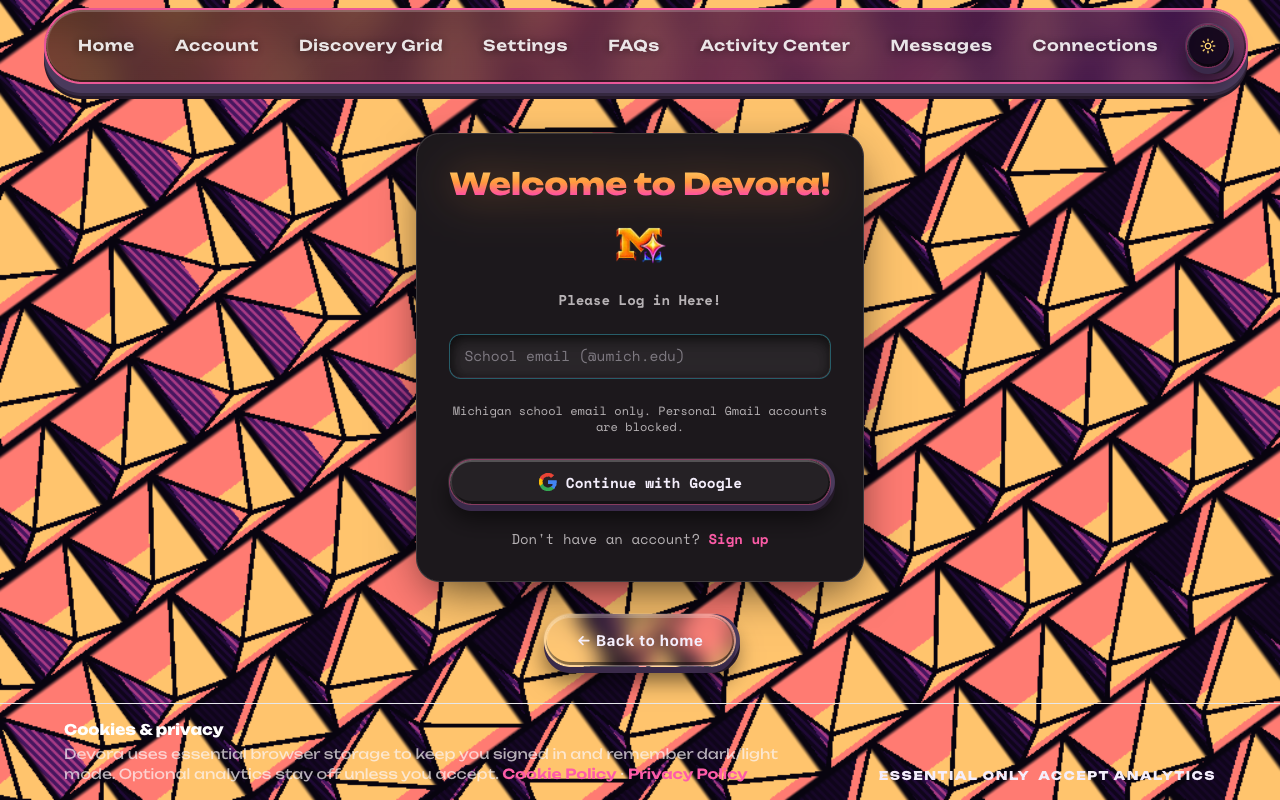
\includegraphics[width=\textwidth]{devora/docs/screenshots/auth-login-desktop.png}
  \caption*{Desktop View (1280px)}
\end{minipage}
\hfill
\begin{minipage}[b]{0.29\textwidth}
  \centering
  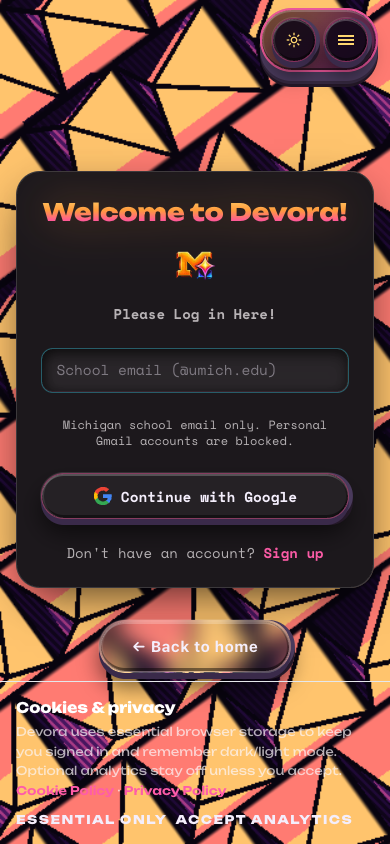
\includegraphics[width=\textwidth]{devora/docs/screenshots/auth-login-mobile.png}
  \caption*{Mobile View (390px)}
\end{minipage}
\caption{Login Interface (\texttt{/auth/login}): Glassmorphic card over procedural shader canvas with institutional email hint, Google Sign-In primary button, and navigation link to signup.}
\label{fig:screen-login}
\end{figure}

\begin{figure}[H]
\centering
\begin{minipage}[b]{0.66\textwidth}
  \centering
  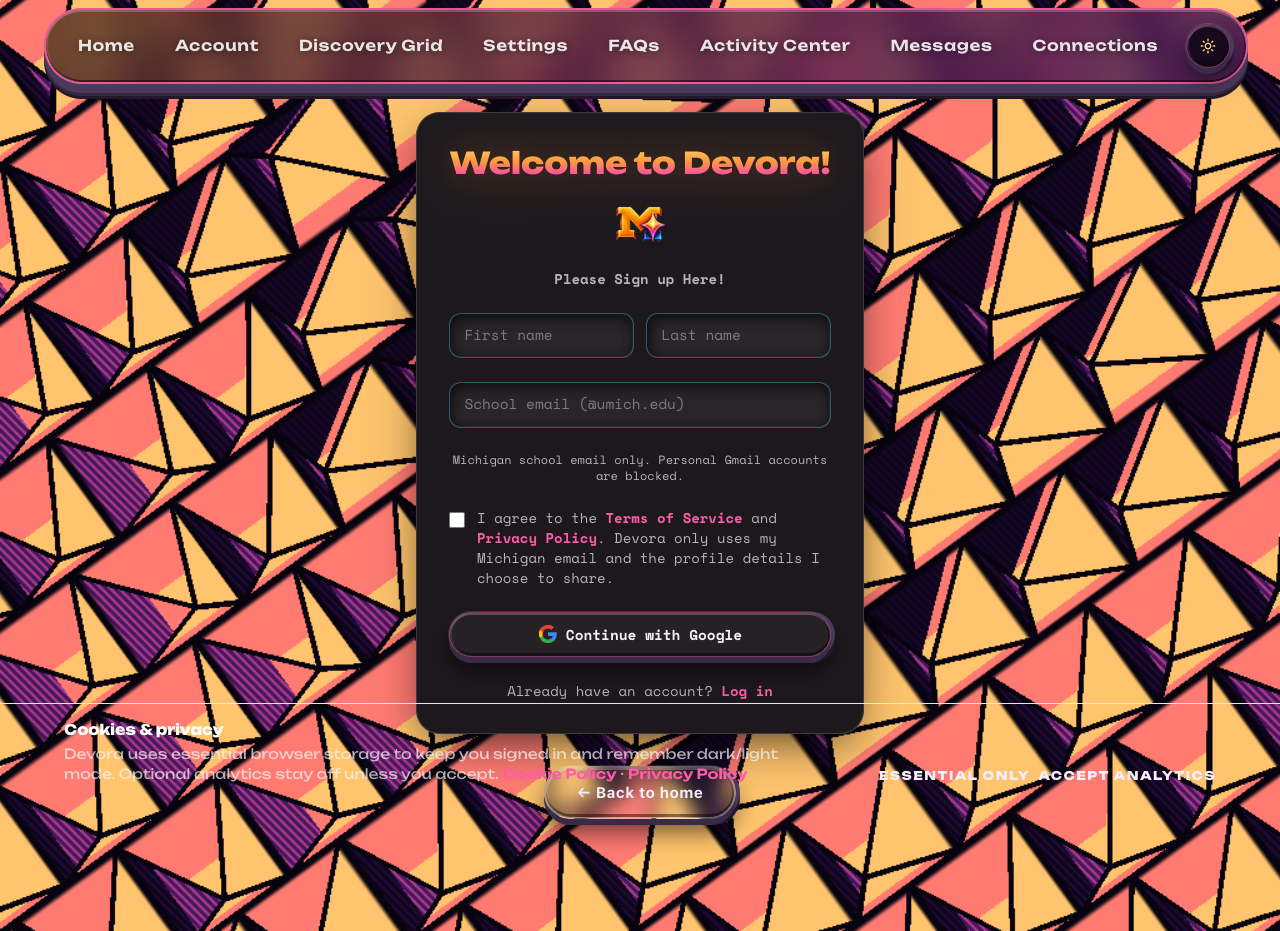
\includegraphics[width=\textwidth]{devora/docs/screenshots/auth-signup-desktop.png}
  \caption*{Desktop View (1280px)}
\end{minipage}
\hfill
\begin{minipage}[b]{0.29\textwidth}
  \centering
  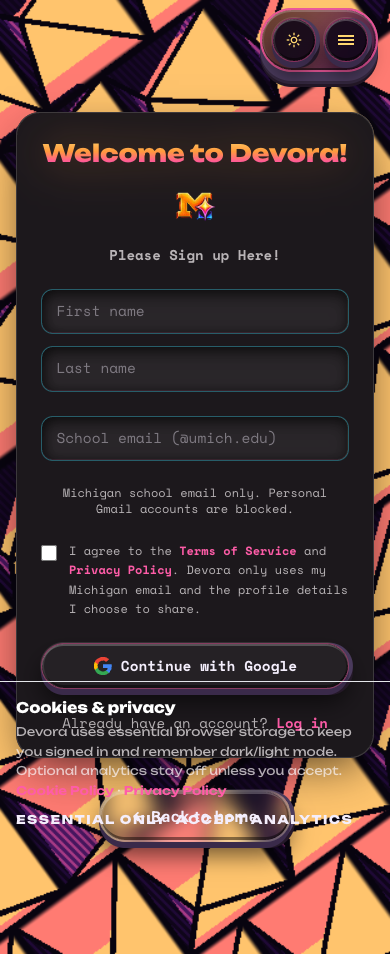
\includegraphics[width=\textwidth]{devora/docs/screenshots/auth-signup-mobile.png}
  \caption*{Mobile View (390px)}
\end{minipage}
\caption{Sign-Up Interface (\texttt{/auth/signup}): Registration card prompting for university Google account, mandatory Terms and Privacy agreement checkboxes, and redirect link to login.}
\label{fig:screen-signup}
\end{figure}

\begin{figure}[H]
\centering
\begin{minipage}[b]{0.66\textwidth}
  \centering
  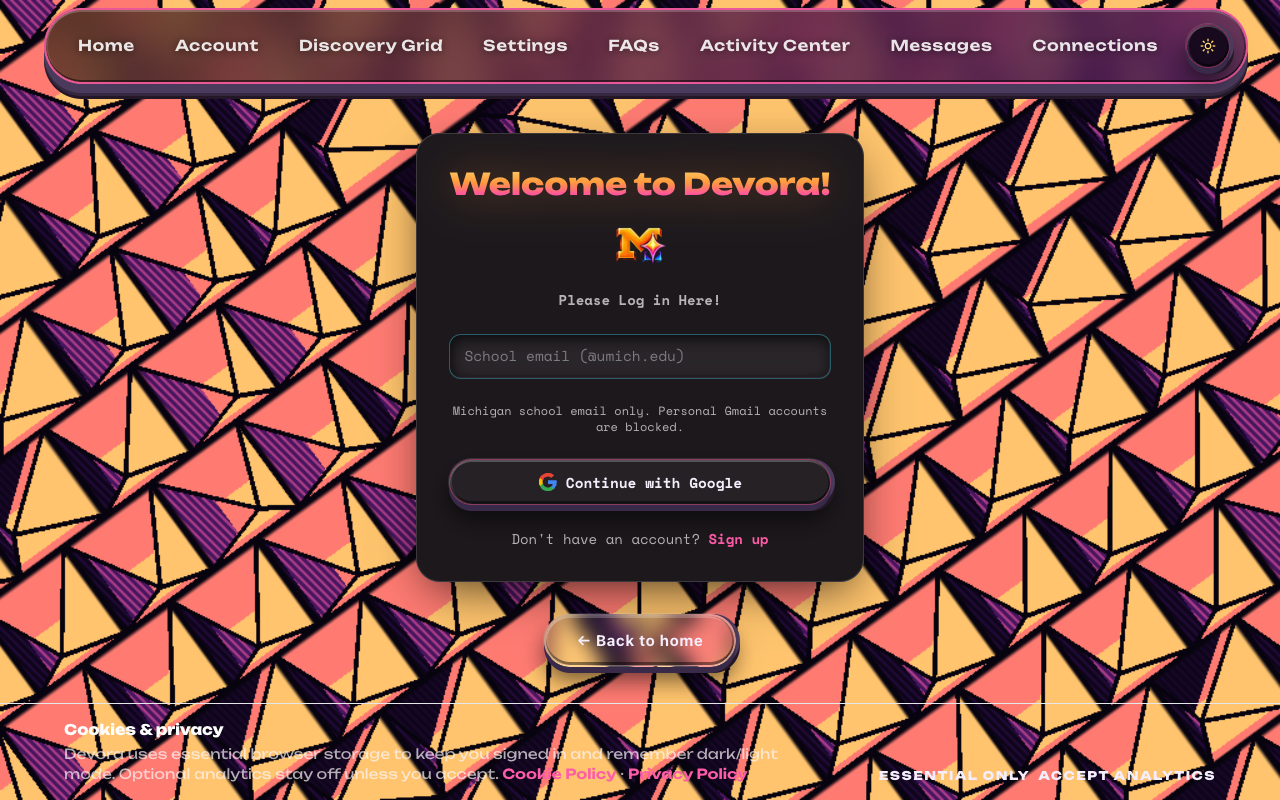
\includegraphics[width=\textwidth]{devora/docs/screenshots/onboarding-desktop.png}
  \caption*{Desktop View (1280px)}
\end{minipage}
\hfill
\begin{minipage}[b]{0.29\textwidth}
  \centering
  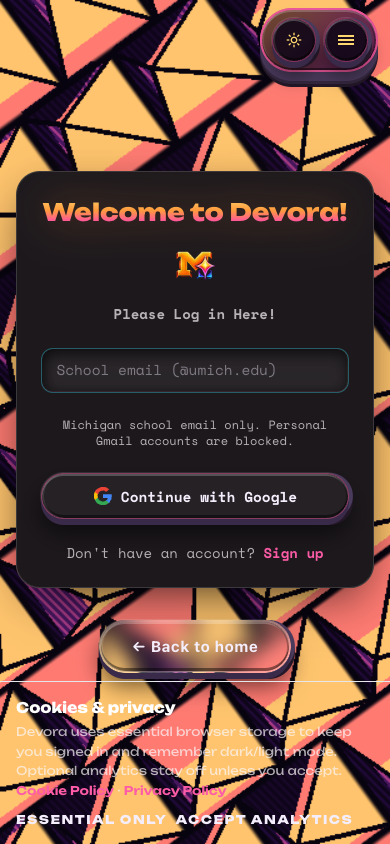
\includegraphics[width=\textwidth]{devora/docs/screenshots/onboarding-mobile.png}
  \caption*{Mobile View (390px)}
\end{minipage}
\caption{Onboarding Wizard (\texttt{/onboarding}): 5-step registration wizard featuring progress step indicators, pill selection buttons for class standing and major, and custom interest inputs.}
\label{fig:screen-onboarding}
\end{figure}

\begin{figure}[H]
\centering
\begin{minipage}[b]{0.66\textwidth}
  \centering
  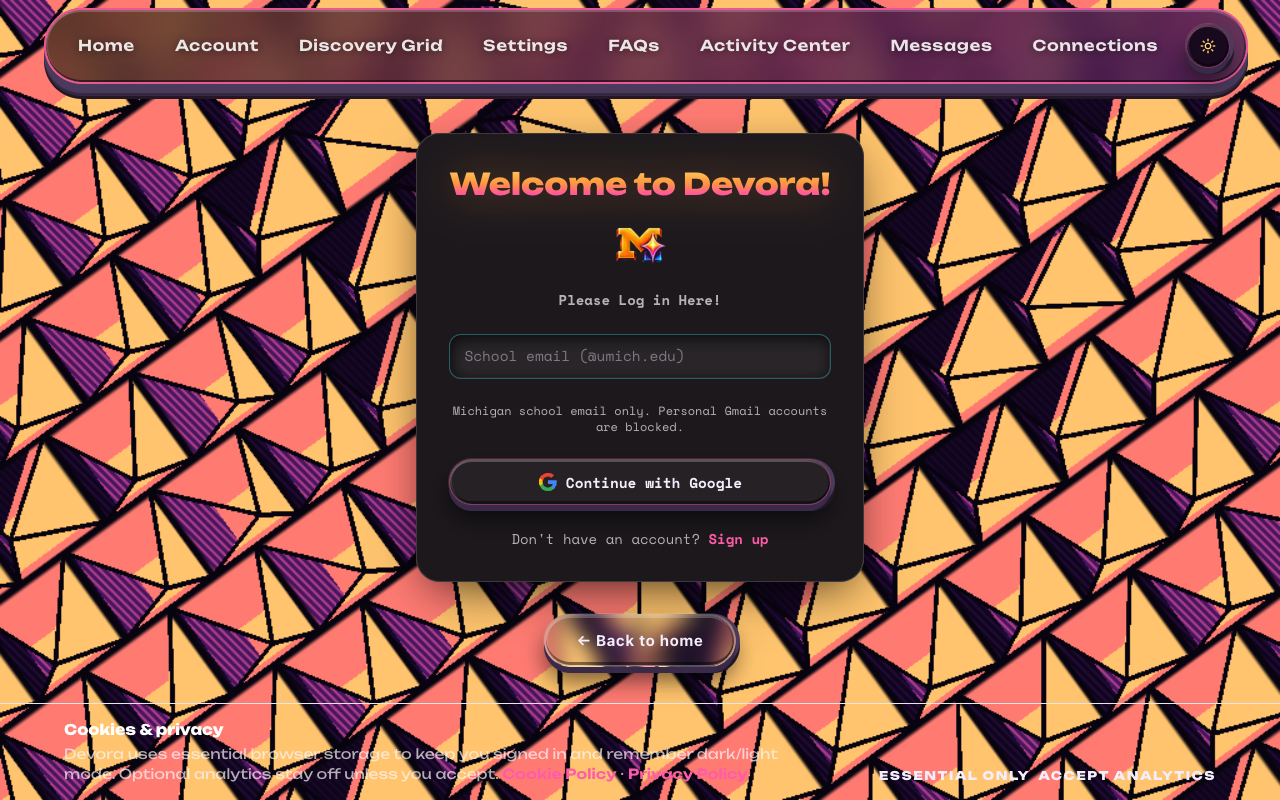
\includegraphics[width=\textwidth]{devora/docs/screenshots/onboarding-welcome-desktop.png}
  \caption*{Desktop View (1280px)}
\end{minipage}
\hfill
\begin{minipage}[b]{0.29\textwidth}
  \centering
  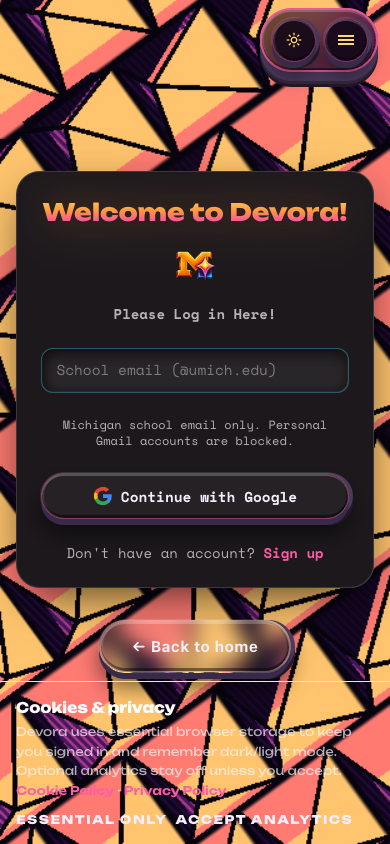
\includegraphics[width=\textwidth]{devora/docs/screenshots/onboarding-welcome-mobile.png}
  \caption*{Mobile View (390px)}
\end{minipage}
\caption{Onboarding Welcome Screen (\texttt{/onboarding/welcome}): Post-registration celebration view confirming profile publication with direct navigation call-to-action to find classmates.}
\label{fig:screen-welcome}
\end{figure}

\begin{figure}[H]
\centering
\begin{minipage}[b]{0.66\textwidth}
  \centering
  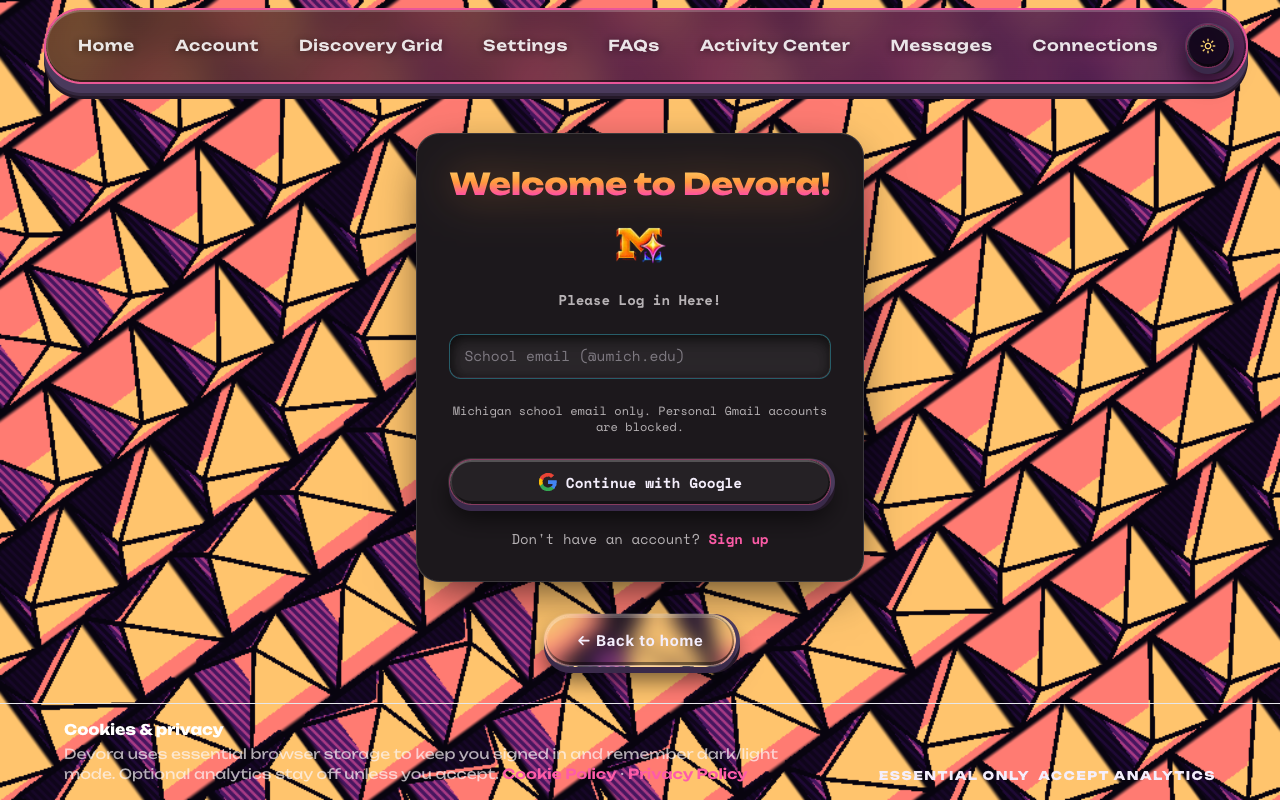
\includegraphics[width=\textwidth]{devora/docs/screenshots/find-students-desktop.png}
  \caption*{Desktop View (1280px)}
\end{minipage}
\hfill
\begin{minipage}[b]{0.29\textwidth}
  \centering
  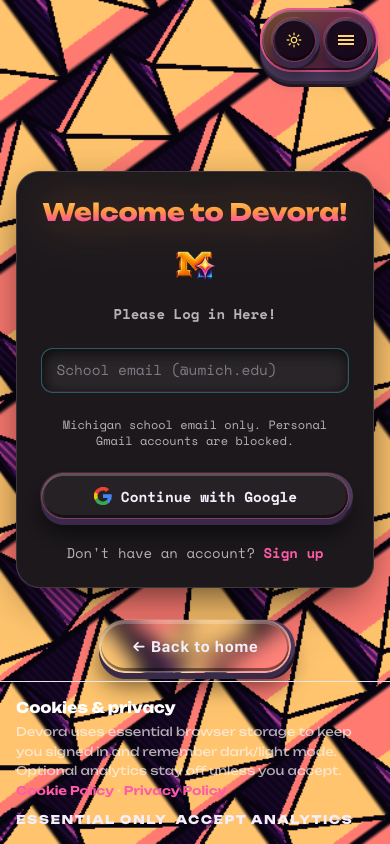
\includegraphics[width=\textwidth]{devora/docs/screenshots/find-students-mobile.png}
  \caption*{Mobile View (390px)}
\end{minipage}
\caption{Discovery Grid Directory (\texttt{/find-students}): Core classmate discovery interface featuring top search input, slide-out multi-criteria filter drawer, active tag filters, and 3-column student card layout.}
\label{fig:screen-find-students}
\end{figure}

\begin{figure}[H]
\centering
\begin{minipage}[b]{0.66\textwidth}
  \centering
  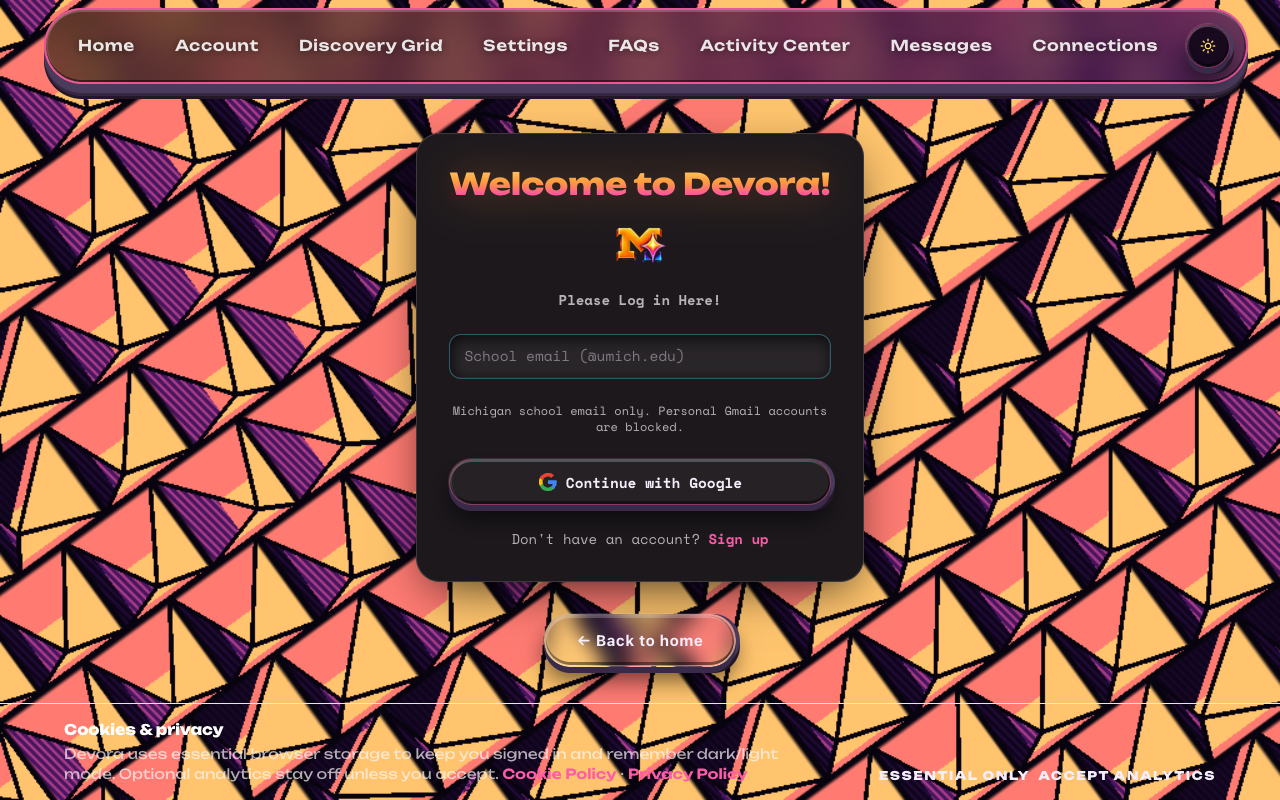
\includegraphics[width=\textwidth]{devora/docs/screenshots/account-page-desktop.png}
  \caption*{Desktop View (1280px)}
\end{minipage}
\hfill
\begin{minipage}[b]{0.29\textwidth}
  \centering
  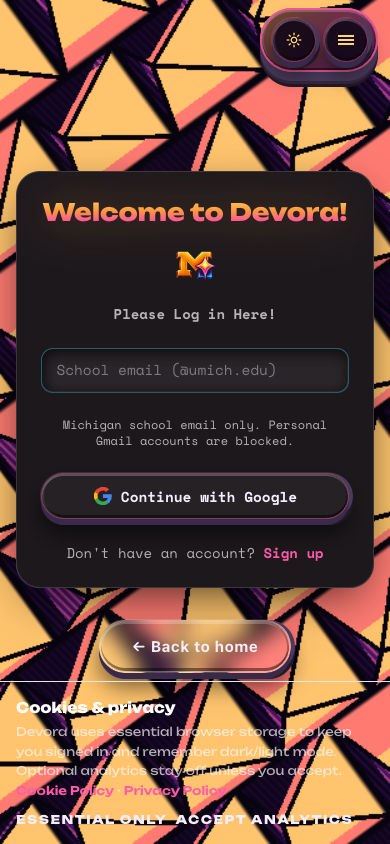
\includegraphics[width=\textwidth]{devora/docs/screenshots/account-page-mobile.png}
  \caption*{Mobile View (390px)}
\end{minipage}
\caption{Account Profile Interface (\texttt{/account-page}): Authenticated profile view showing user avatar with gradient halo, profile completeness meter, academic badges, public card preview, and edit modal trigger.}
\label{fig:screen-account}
\end{figure}

\begin{figure}[H]
\centering
\begin{minipage}[b]{0.66\textwidth}
  \centering
  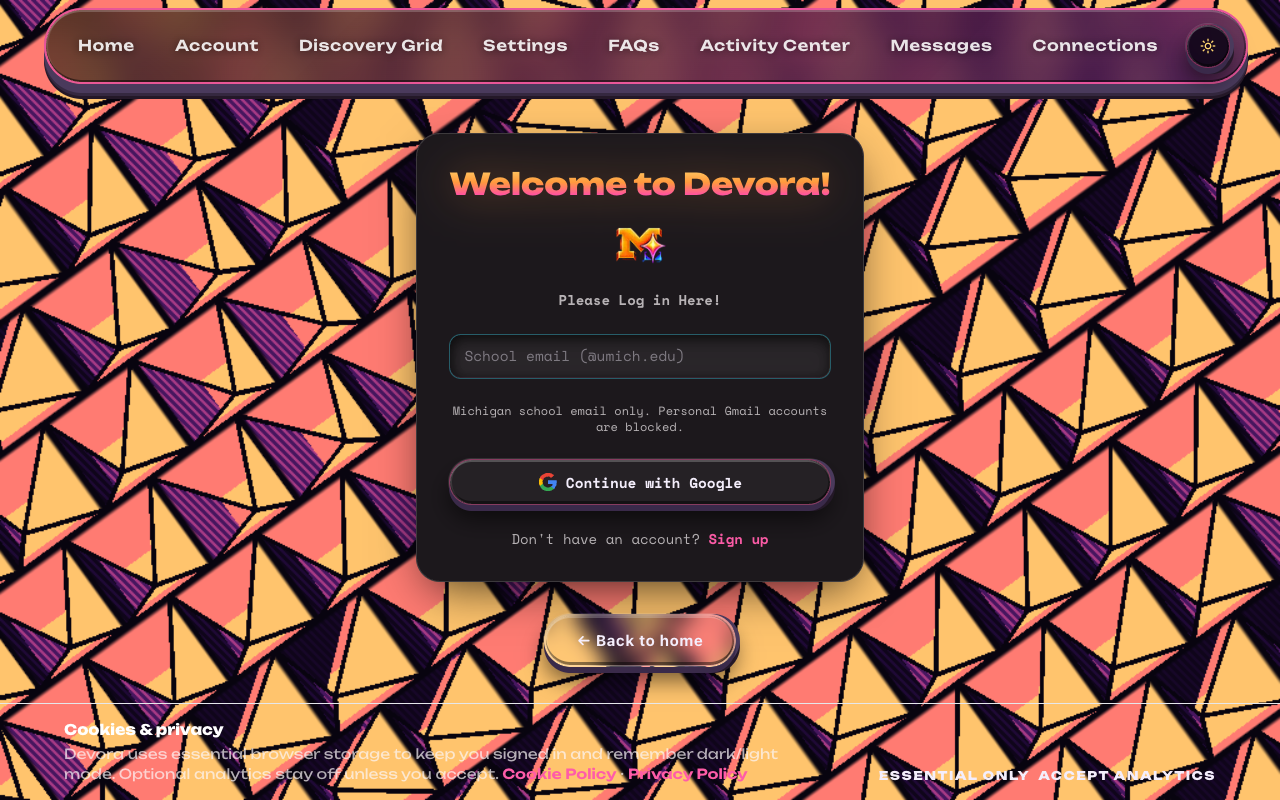
\includegraphics[width=\textwidth]{devora/docs/screenshots/settings-desktop.png}
  \caption*{Desktop View (1280px)}
\end{minipage}
\hfill
\begin{minipage}[b]{0.29\textwidth}
  \centering
  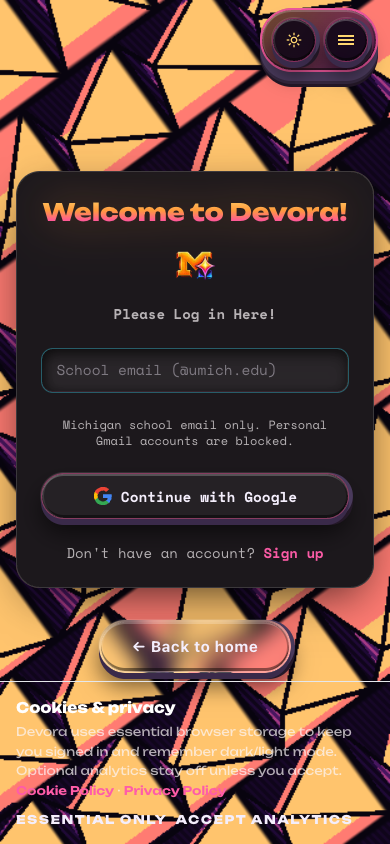
\includegraphics[width=\textwidth]{devora/docs/screenshots/settings-mobile.png}
  \caption*{Mobile View (390px)}
\end{minipage}
\caption{Settings Interface (\texttt{/settings}): Configuration panel featuring 11 granular toggles for visibility, search index inclusion, notification channels, and destructive Danger Zone controls.}
\label{fig:screen-settings}
\end{figure}

\begin{figure}[H]
\centering
\begin{minipage}[b]{0.66\textwidth}
  \centering
  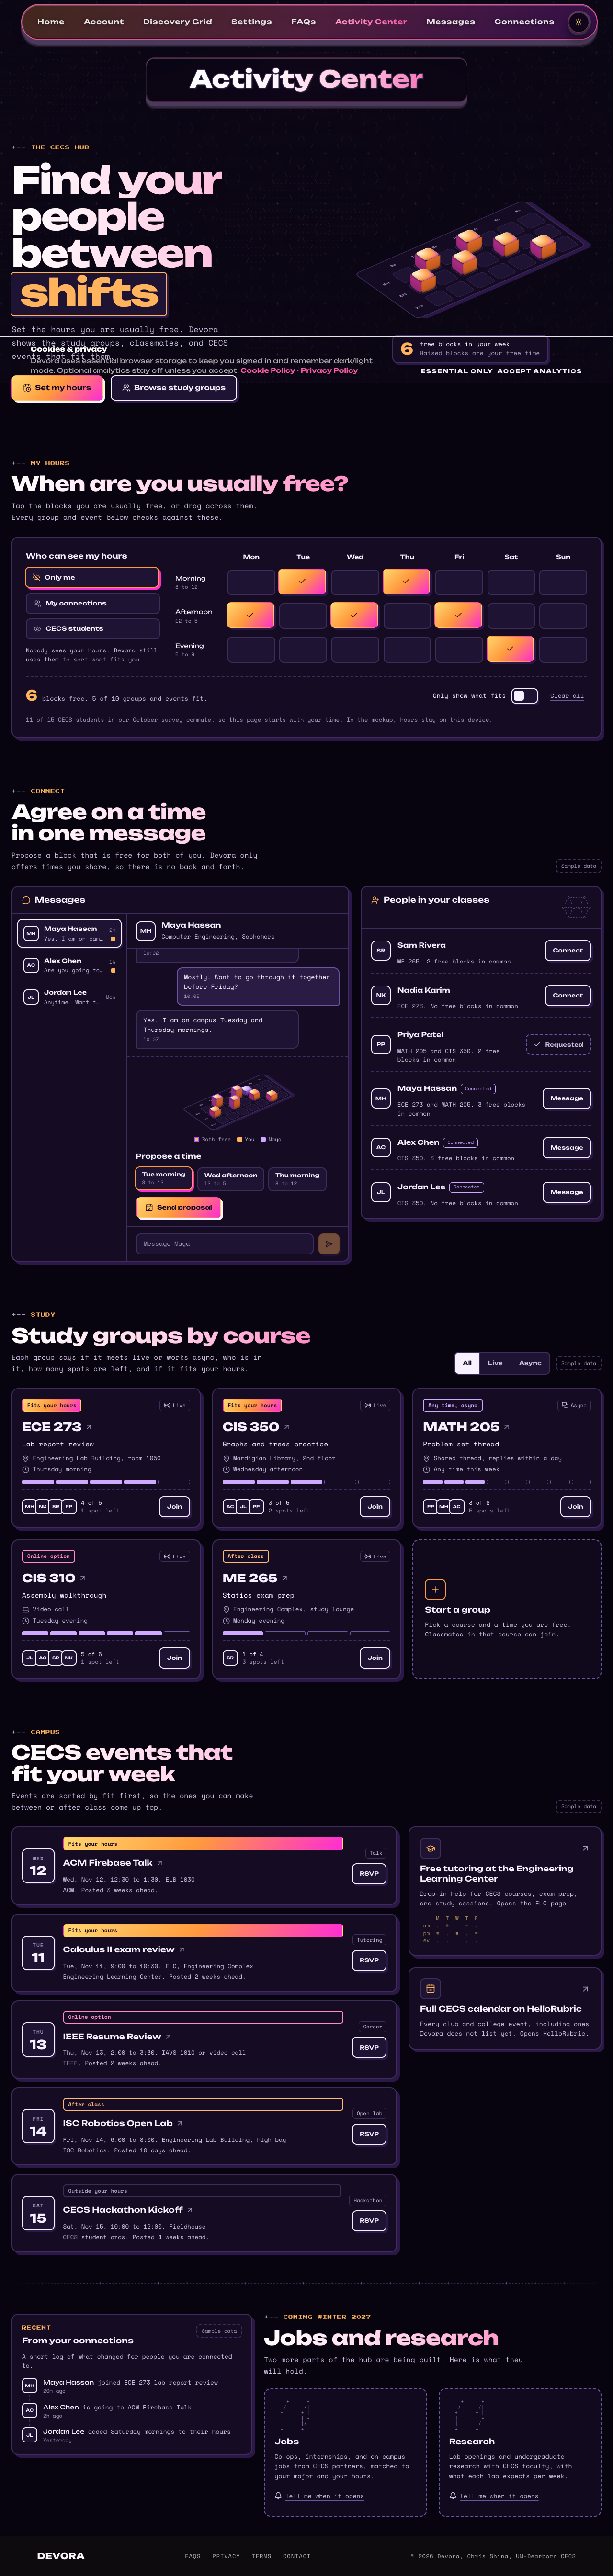
\includegraphics[width=\textwidth]{devora/docs/screenshots/messages-page-desktop.png}
  \caption*{Desktop View (1280px)}
\end{minipage}
\hfill
\begin{minipage}[b]{0.29\textwidth}
  \centering
  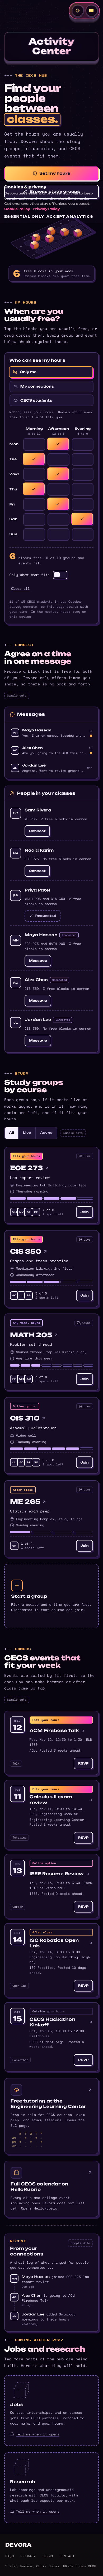
\includegraphics[width=\textwidth]{devora/docs/screenshots/messages-page-mobile.png}
  \caption*{Mobile View (390px)}
\end{minipage}
\caption{Activity Center Interface (\texttt{/messages-page}): Interactive shell displaying weekly availability scheduling matrix, message threads, study group hubs, and campus event feeds.}
\label{fig:screen-messages}
\end{figure}

\begin{figure}[H]
\centering
\begin{minipage}[b]{0.66\textwidth}
  \centering
  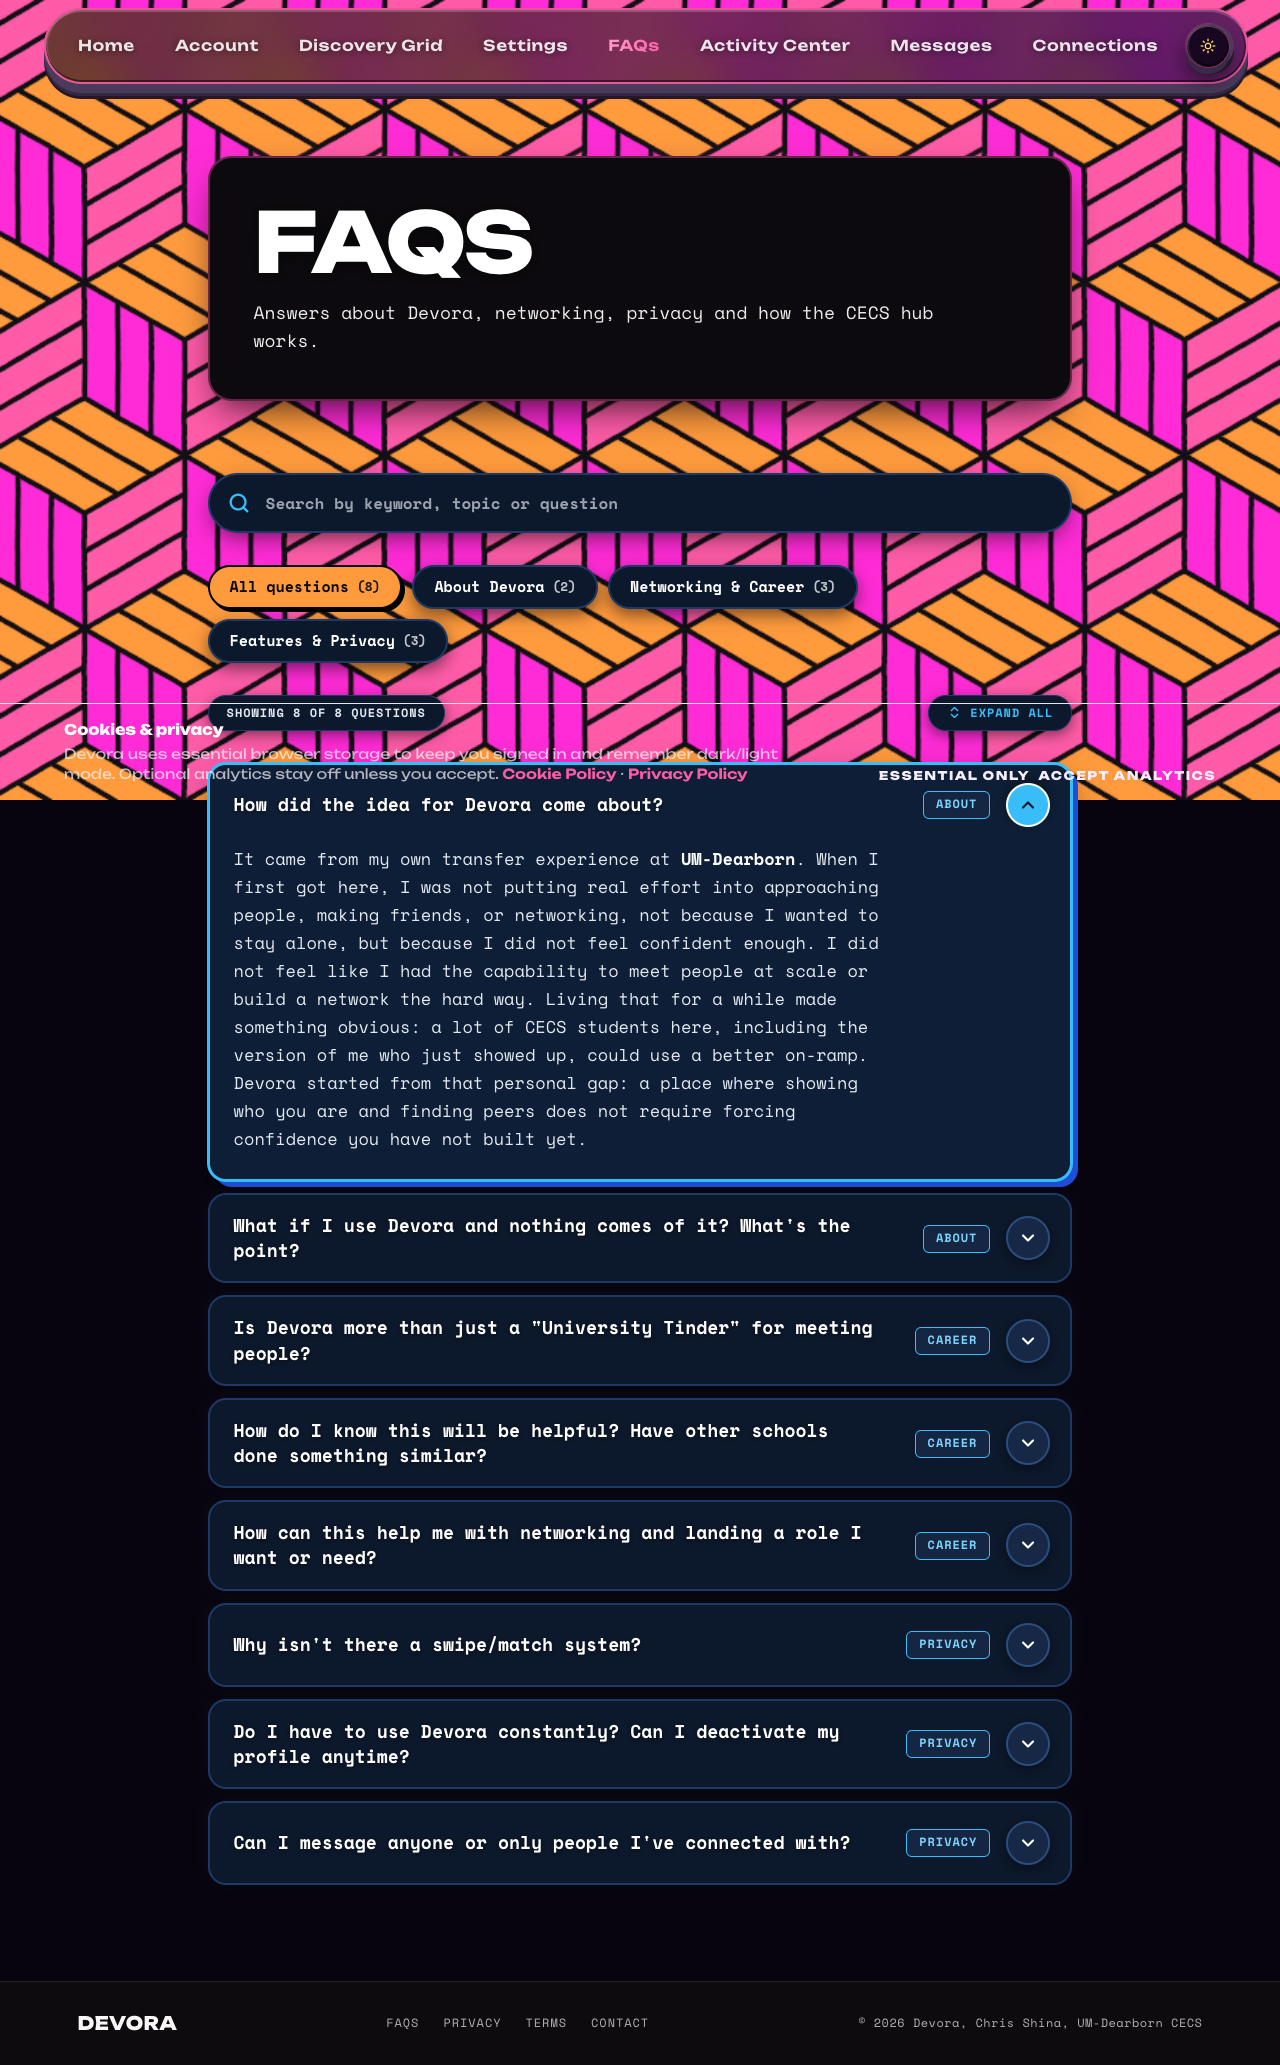
\includegraphics[width=\textwidth]{devora/docs/screenshots/faqs-page-desktop.png}
  \caption*{Desktop View (1280px)}
\end{minipage}
\hfill
\begin{minipage}[b]{0.29\textwidth}
  \centering
  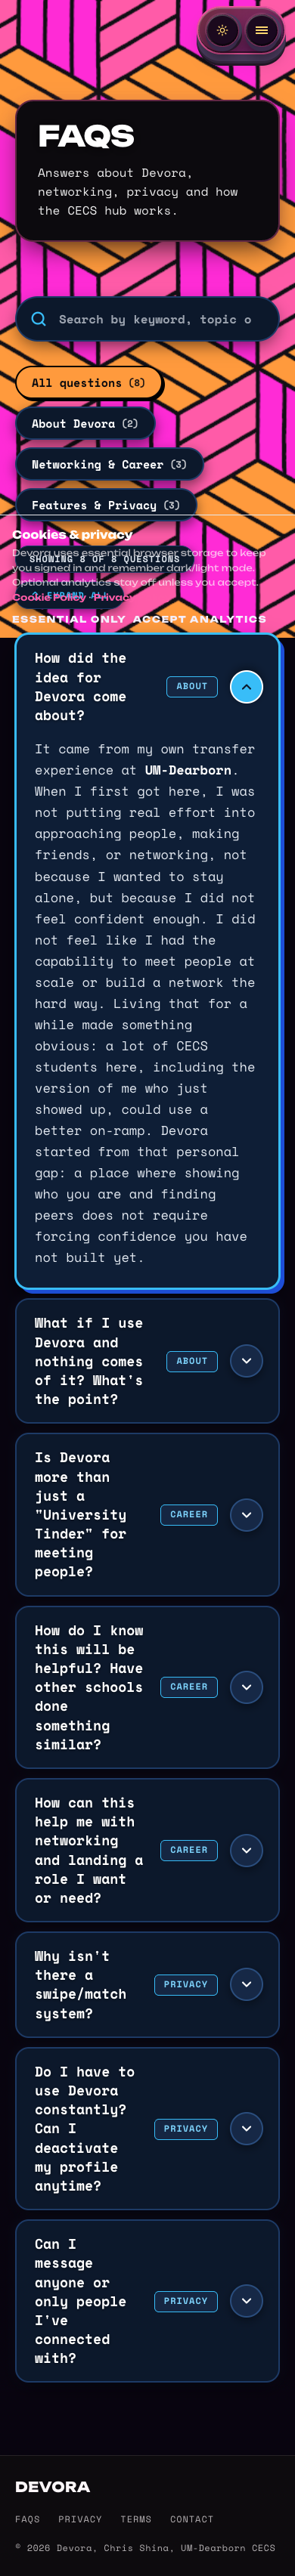
\includegraphics[width=\textwidth]{devora/docs/screenshots/faqs-page-mobile.png}
  \caption*{Mobile View (390px)}
\end{minipage}
\caption{Frequently Asked Questions (\texttt{/faqs-page}): Searchable accordion component over geometric background, categorizing questions across platform features, privacy policies, and CECS guidelines.}
\label{fig:screen-faqs}
\end{figure}

\begin{figure}[H]
\centering
\begin{minipage}[b]{0.66\textwidth}
  \centering
  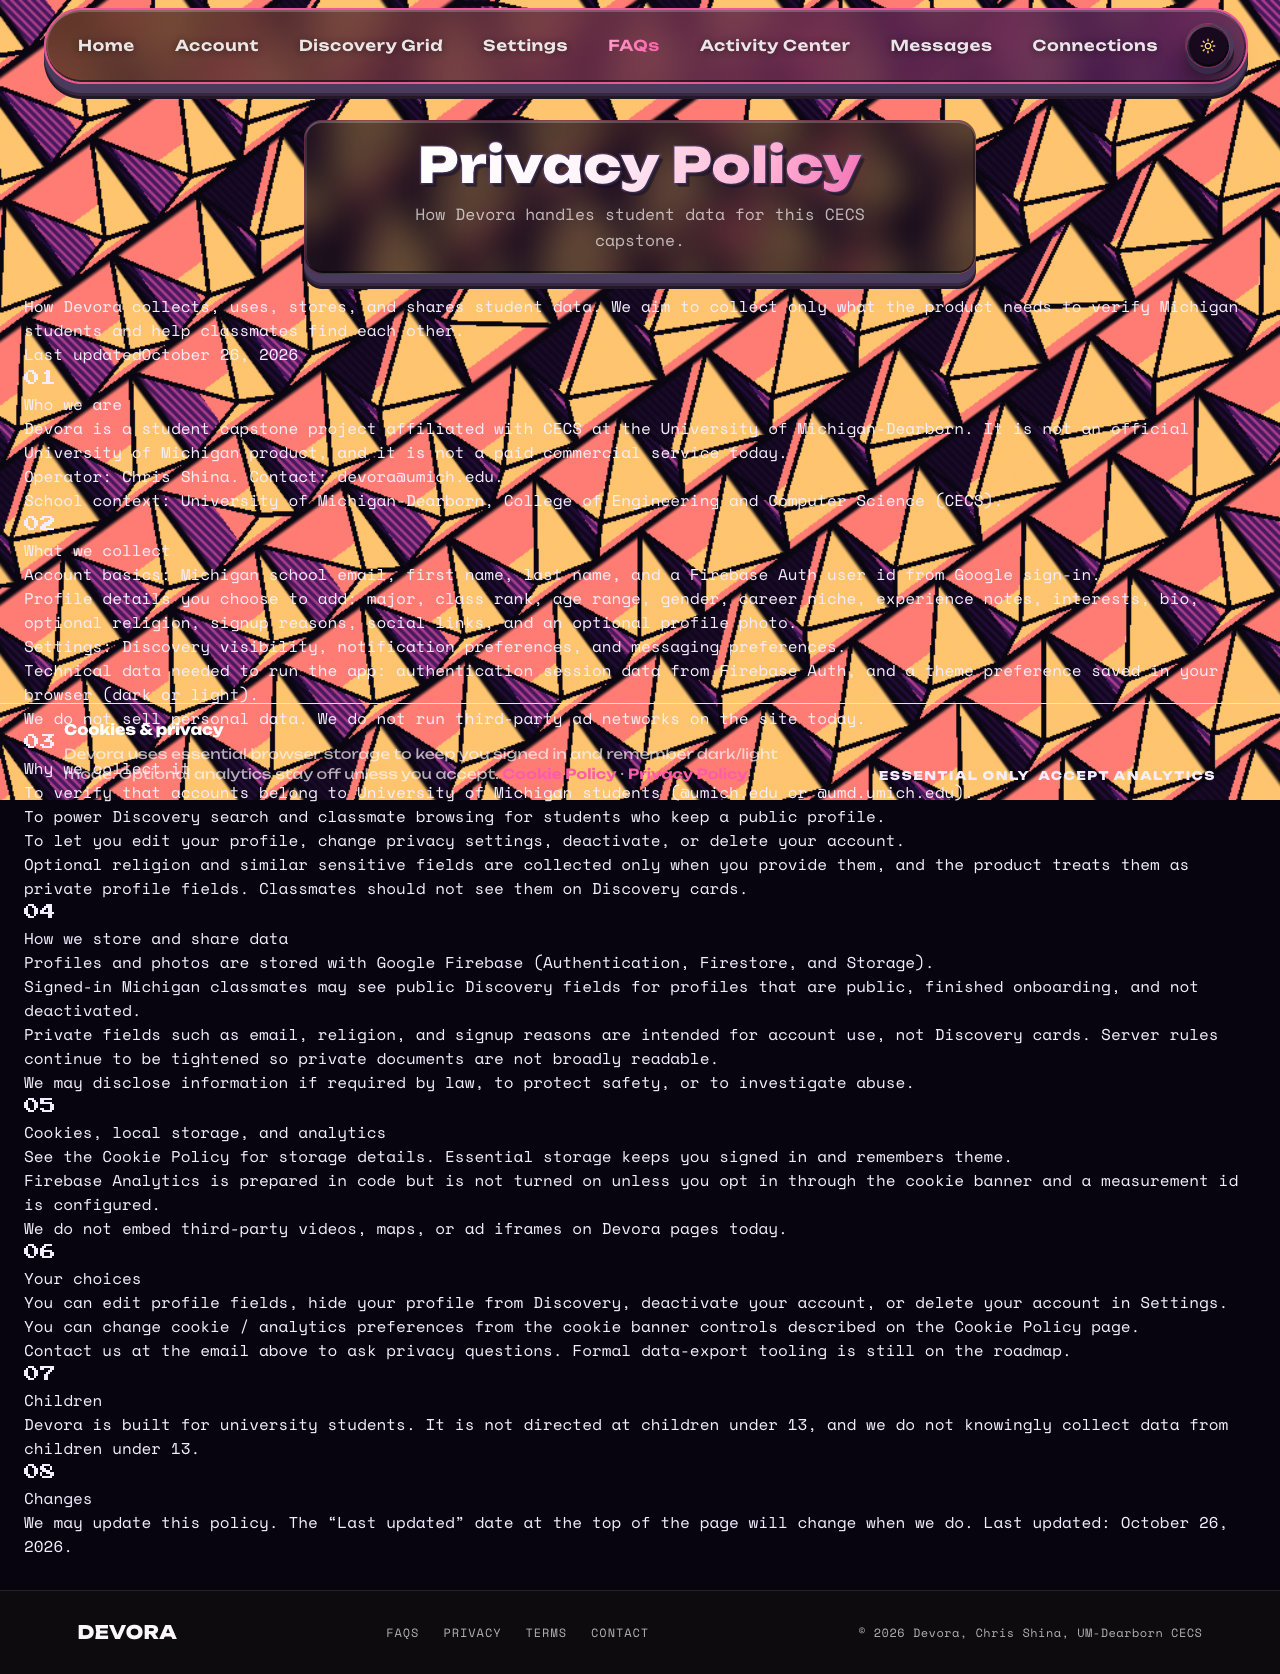
\includegraphics[width=\textwidth]{devora/docs/screenshots/privacy-page-desktop.png}
  \caption*{Desktop View (1280px)}
\end{minipage}
\hfill
\begin{minipage}[b]{0.29\textwidth}
  \centering
  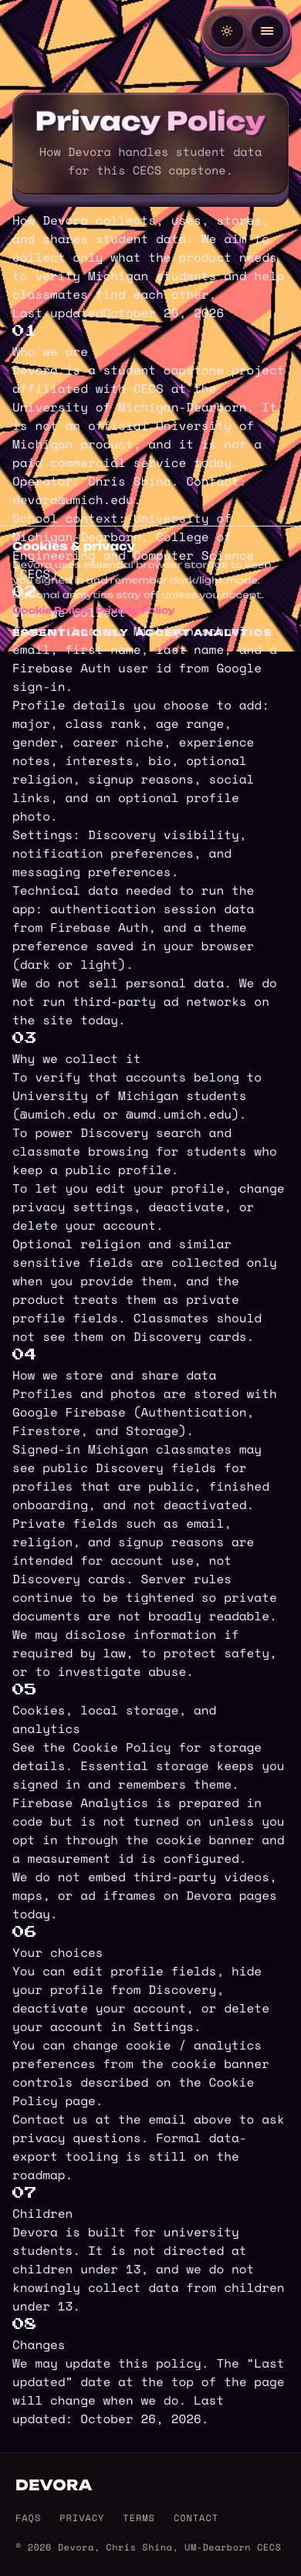
\includegraphics[width=\textwidth]{devora/docs/screenshots/privacy-page-mobile.png}
  \caption*{Mobile View (390px)}
\end{minipage}
\caption{Privacy Policy (\texttt{/privacy-page}): Institutional data protection notice detailing voluntary directory participation, FERPA boundary guarantees, and private data handling.}
\label{fig:screen-privacy}
\end{figure}

\begin{figure}[H]
\centering
\begin{minipage}[b]{0.66\textwidth}
  \centering
  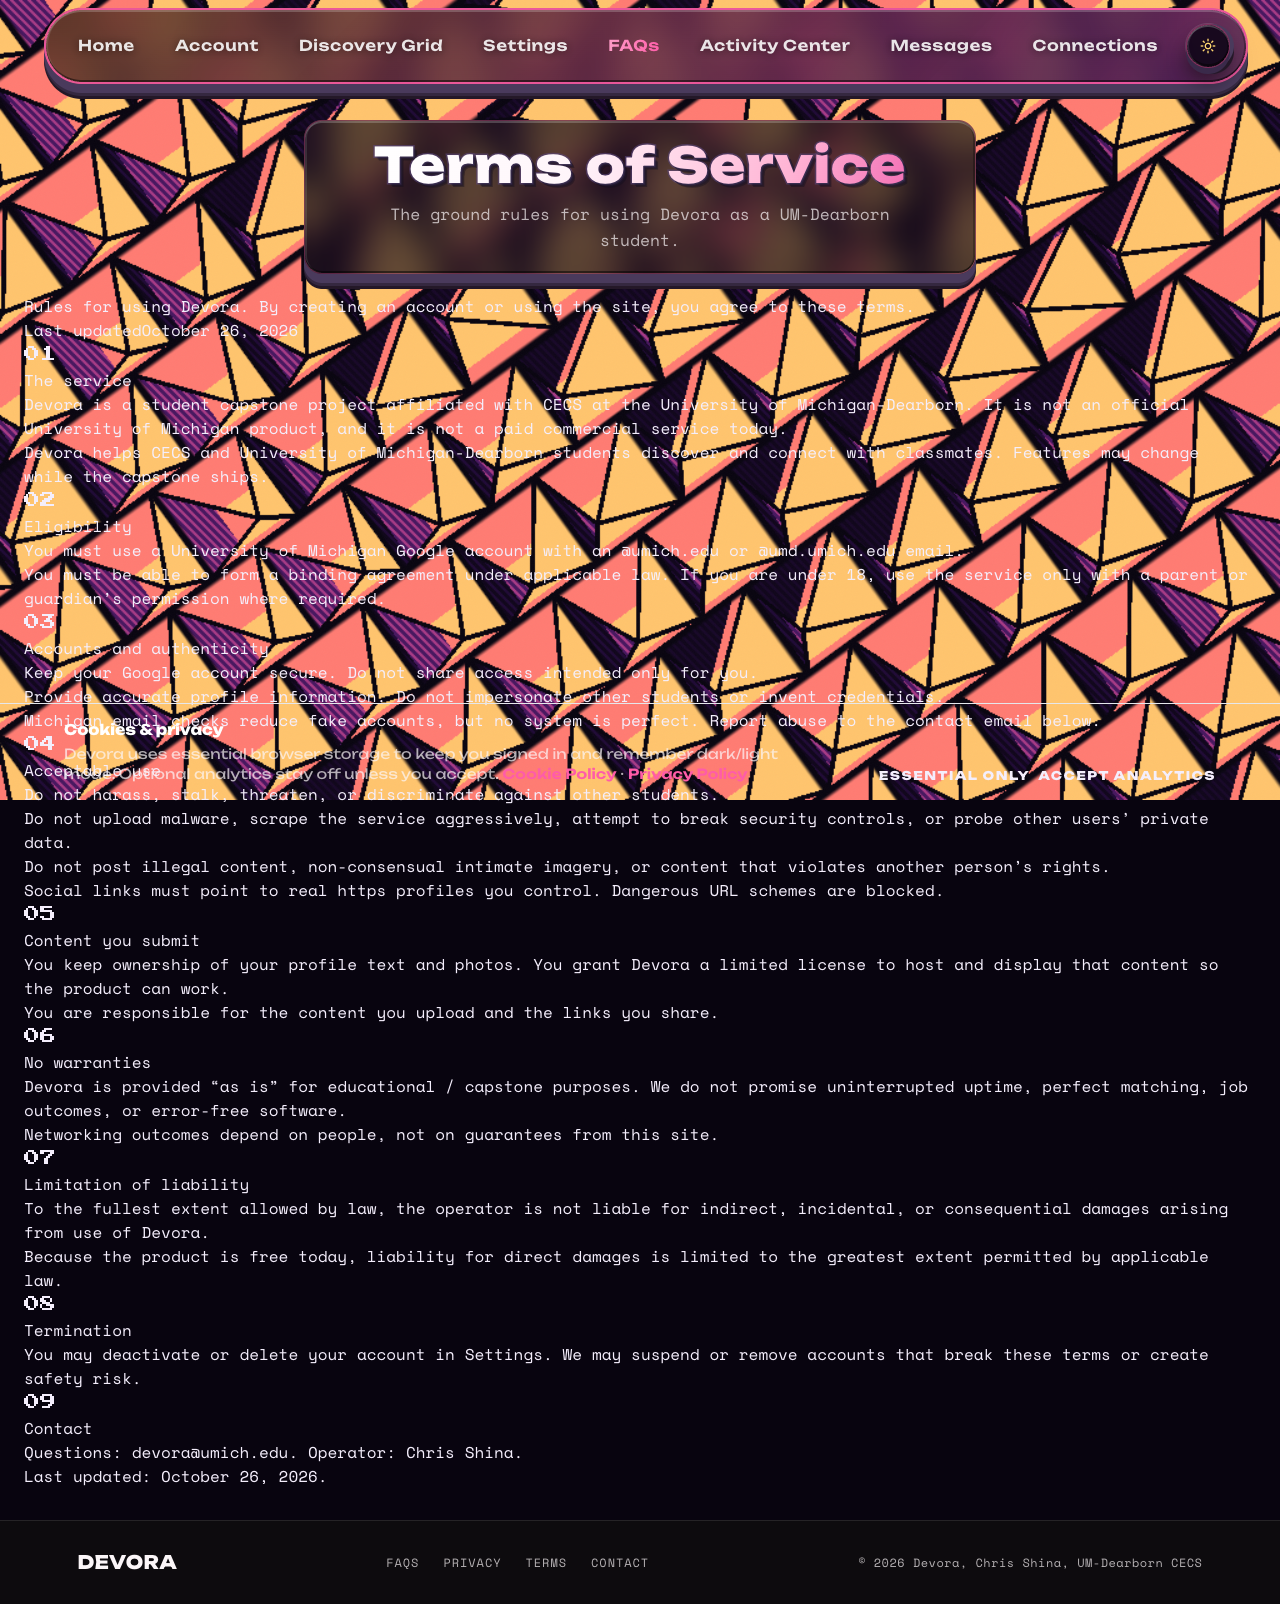
\includegraphics[width=\textwidth]{devora/docs/screenshots/terms-page-desktop.png}
  \caption*{Desktop View (1280px)}
\end{minipage}
\hfill
\begin{minipage}[b]{0.29\textwidth}
  \centering
  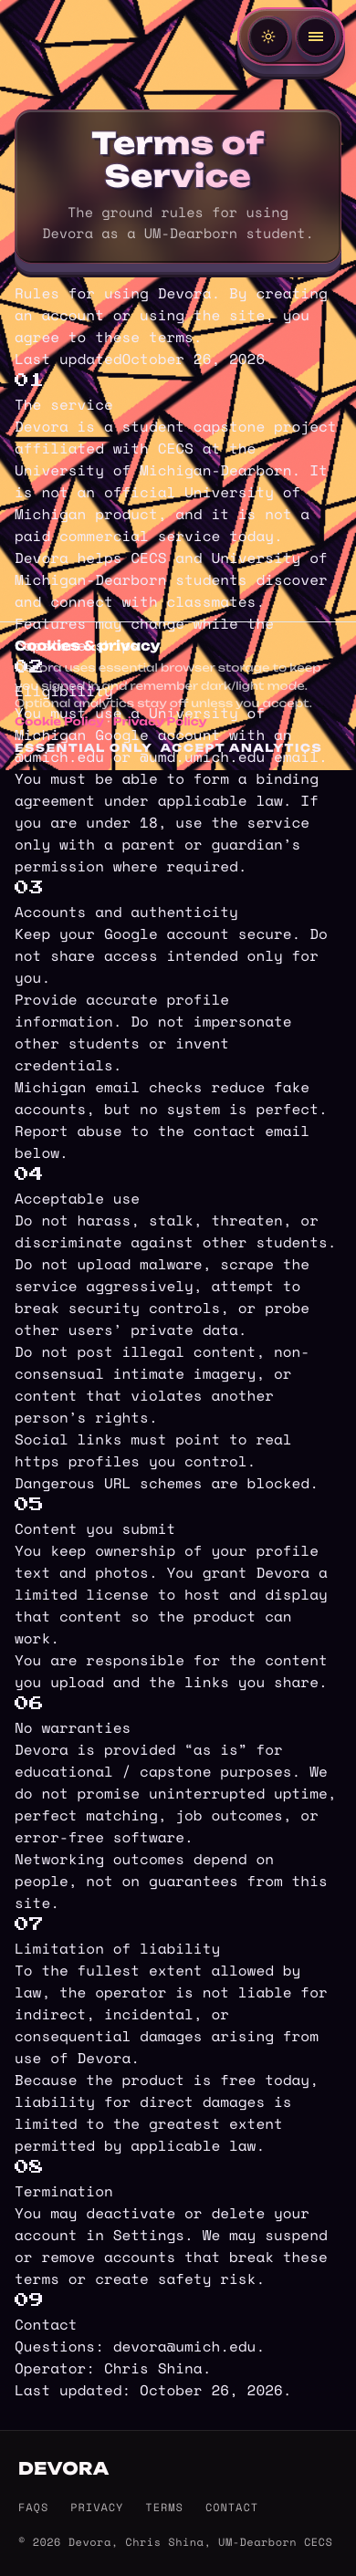
\includegraphics[width=\textwidth]{devora/docs/screenshots/terms-page-mobile.png}
  \caption*{Mobile View (390px)}
\end{minipage}
\caption{Terms of Service (\texttt{/terms-page}): User agreement outlining community conduct standards, student affiliation requirements, and acceptable use within CECS.}
\label{fig:screen-terms}
\end{figure}

\begin{figure}[H]
\centering
\begin{minipage}[b]{0.66\textwidth}
  \centering
  
\includegraphics[width=\textwidth]{devora/docs/screenshots/cookies-page-desktop.png}
  \caption*{Desktop View (1280px)}
\end{minipage}
\hfill
\begin{minipage}[b]{0.29\textwidth}
  \centering
  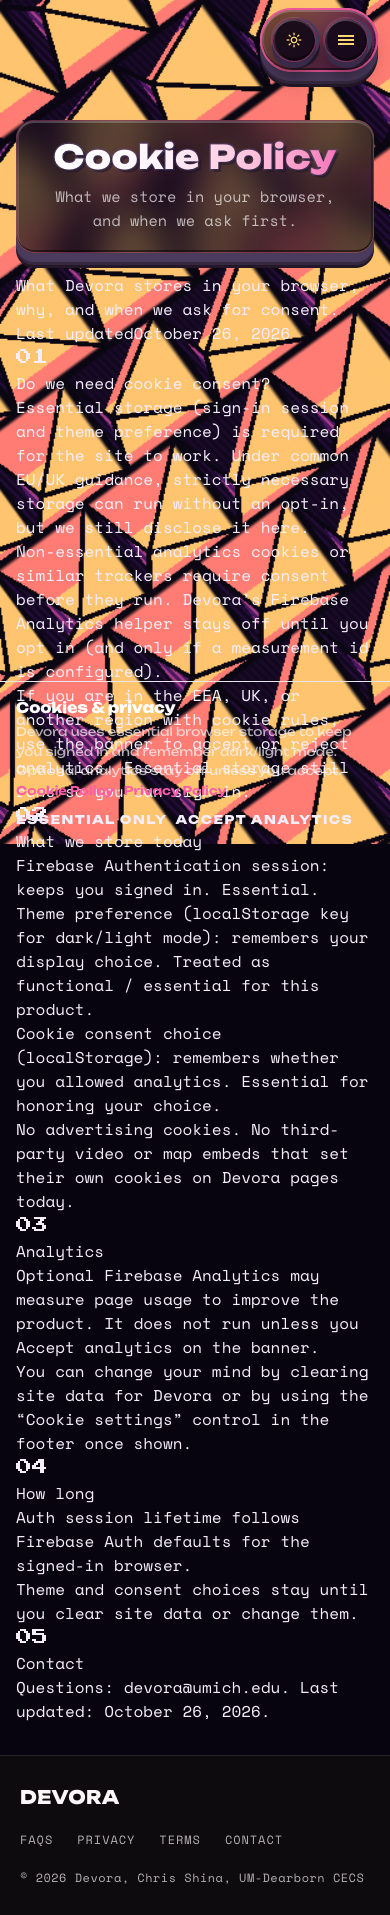
\includegraphics[width=\textwidth]{devora/docs/screenshots/cookies-page-mobile.png}
  \caption*{Mobile View (390px)}
\end{minipage}
\caption{Cookie Policy (\texttt{/cookies-page}): Technical compliance disclosure defining essential session tokens versus optional analytics cookies and consent mechanics.}
\label{fig:screen-cookies}
\end{figure}

\begin{figure}[H]
\centering
\begin{minipage}[b]{0.66\textwidth}
  \centering
  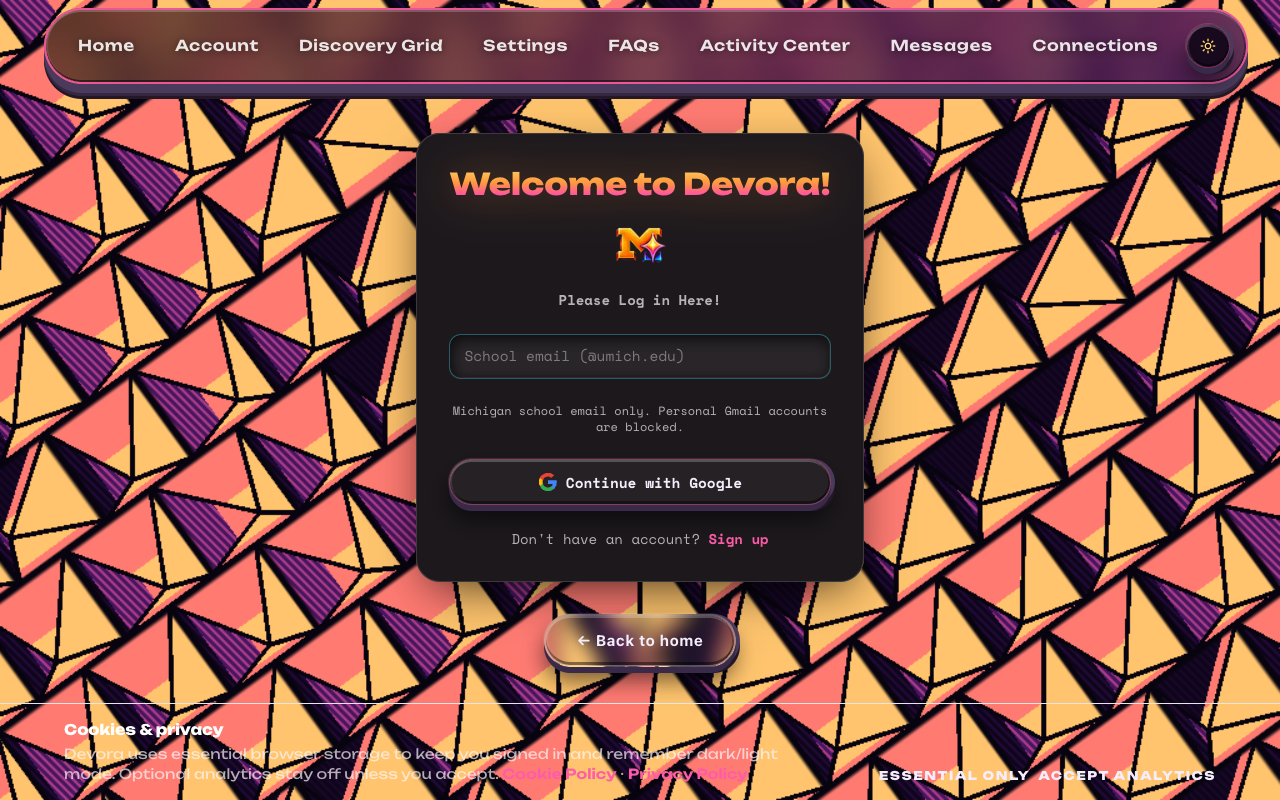
\includegraphics[width=\textwidth]{devora/docs/screenshots/auth-deactivated-desktop.png}
  \caption*{Desktop View (1280px)}
\end{minipage}
\hfill
\begin{minipage}[b]{0.29\textwidth}
  \centering
  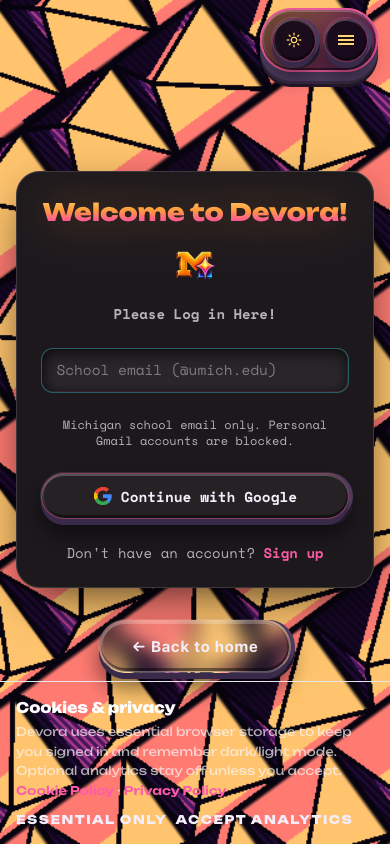
\includegraphics[width=\textwidth]{devora/docs/screenshots/auth-deactivated-mobile.png}
  \caption*{Mobile View (390px)}
\end{minipage}
\caption{Deactivated Notice Interface (\texttt{/auth/deactivated}): Account state screen informing the user their profile is hidden from discovery with a one-click reactivation action button.}
\label{fig:screen-deactivated}
\end{figure}

\subsubsection*{4.1.2 Objects and actions}

\begin{table}[h!]
\centering
\small
\begin{tabularx}{\textwidth}{p{3.2cm} p{2.2cm} Y}
\toprule
\textbf{Route} & \textbf{Status} & \textbf{Authentication and Access Guard} \\
\midrule
\texttt{/} & \texttt{BUILT} & Redirects immediately to \texttt{/home}. \\
\texttt{/home} & \texttt{BUILT} & Public; no sign-in check. \\
\texttt{/auth/login}, \texttt{/auth/signup} & \texttt{BUILT} & Public; redirects to \texttt{/find-students} if already signed in. \\
\texttt{/auth/deactivated} & \texttt{BUILT} & Client-guarded; redirects if signed out or account active. \\
\texttt{/onboarding}, \texttt{/onboarding/welcome} & \texttt{BUILT} & Client-guarded; redirects to \texttt{/auth/login} if signed out. \\
\texttt{/account-page} & \texttt{BUILT} & Client-guarded; redirects if signed out or not onboarded. \\
\texttt{/settings} & \texttt{BUILT} & Client-guarded; redirects to \texttt{/auth/login} if signed out. \\
\texttt{/faqs-page} & \texttt{BUILT} & Public; no sign-in check. \\
\texttt{/find-students} (Discovery Grid) & \texttt{BUILT} & \textbf{Client-guarded}; redirects to \texttt{/auth/login} if signed out and to \texttt{/onboarding} if not onboarded. \\
\texttt{/messages-page} (Activity Center) & \texttt{PARTIAL} & Public preview shell; live backend guard planned. \\
\texttt{/privacy-page}, \texttt{/terms-page}, \texttt{/cookies-page} & \texttt{BUILT} & Public compliance documents; no sign-in check. \\
\bottomrule
\end{tabularx}
\end{table}

\subsection*{4.2 Interface design rules}
\begin{itemize}[leftmargin=*,itemsep=3pt]
\item \textbf{Typography:} The application utilizes three distinct Google web font families loaded via \texttt{next/font/google} in \texttt{src/app/layout.tsx}:
  \begin{itemize}[noitemsep]
  \item \textbf{Space Mono (\texttt{--font-mono}):} Primary monospace typeface for body text, form labels, metadata chips, filter pills, and navigation elements.
  \item \textbf{Unbounded (\texttt{--font-display}):} Geometric display typeface used for all major section headers, hero titles, and branding wordmarks.
  \item \textbf{Press Start 2P (\texttt{--font-pixel}):} Retro 8-bit pixel typeface used for decorative badge accents and gaming-inspired UI details.
  \end{itemize}
  \textit{(Note: Earlier design references to Inter and JetBrains Mono are obsolete; the production codebase uses Space Mono and Unbounded.)}
\item \textbf{Color Palette:} Defined in \texttt{src/ui/globals.css} around a midnight synthwave foundation:
  \begin{itemize}[noitemsep]
  \item Page backgrounds: \texttt{--page-bg: \#08040f}, \texttt{--section-bg: \#08040f}, and \texttt{--section-bg-alt: \#0a0512}.
  \item Text hierarchy: \texttt{--text-primary: \#f4eefc}, \texttt{--heading-color: \#ffffff}, \texttt{--text-body: rgba(255, 255, 255, 0.88)}, and \texttt{--text-muted: rgba(255, 255, 255, 0.6)}.
  \item Glassmorphism: \texttt{--surface-glass: rgba(14, 8, 24, 0.72)} with backdrop blur and border accents \texttt{--border-subtle: rgba(255, 255, 255, 0.08)}.
  \end{itemize}
\item \textbf{Brand Gradients:}
  \begin{itemize}[noitemsep]
  \item Signature gradient: \texttt{--grad: linear-gradient(120deg, \#ff9a3d 0\%, \#ff5ca8 52\%, \#ff2bd6 100\%)}.
  \item Ember gradient: \texttt{--grad-ember: linear-gradient(135deg, \#ff7a18 0\%, \#ff3d77 100\%)}.
  \item Pink gradient: \texttt{--grad-pink: linear-gradient(135deg, \#ff5ca8 0\%, \#ff2bd6 100\%)}.
  \end{itemize}
\item \textbf{3D Button Stacks:} Interactive CTAs use layered offset shadow stacks for tactile depth:
  \begin{itemize}[noitemsep]
  \item Primary CTA: \texttt{--btn-3d-stack: 0 4px 0 \#b33900, 0 8px 24px rgba(255, 92, 168, 0.35)}.
  \item Accent CTA: \texttt{--btn-3d-stack-pink: 0 4px 0 \#990066, 0 8px 24px rgba(255, 43, 214, 0.35)}.
  \end{itemize}
\item \textbf{Accessibility:} Focus outlines utilize \texttt{outline: 2px solid \#ff5ca8}; all interactive animations strictly honor the \texttt{prefers-reduced-motion: reduce} media query.
\end{itemize}

\subsection*{4.3 Components available}
Reusable components located in \texttt{src/ui/}: \texttt{NavBar}, \texttt{Footer}, \texttt{BackgroundPicture} (procedural GLSL shader canvas), \texttt{DiscoveryProfileCard}, \texttt{DiscoveryProfilePeek}, \texttt{DiscoveryFilterSidebar}, \texttt{DiscoveryEmptyState}, \texttt{IsometricEmptyDrawing}, \texttt{AccountProfileEditor}, \texttt{AccountProfileView}, \texttt{SettingsPageContent}, \texttt{FAQAccordion}, \texttt{CookieConsentBanner}, and \texttt{PillSelector}.

\subsection*{4.4 UIDS description}
Devora utilizes standard modern web technologies without a proprietary UI development system: Next.js 14 App Router, React 18 client components, Tailwind CSS utility architecture, Framer Motion for layout transitions, and HTML5 WebGL/Canvas shaders.

\newpage
\section*{5.0 Restrictions, Limitations, and Constraints}

\begin{enumerate}[leftmargin=*,itemsep=4pt]
\item \textbf{Strict Institutional Email Gating:} Access requires an authenticated Google account ending with \texttt{@umich.edu} or \texttt{@umd.umich.edu}. Enforced synchronously across client-side forms, server-side Cloud Functions, and Firestore security rules.
\item \textbf{Data Minimization and Sensitive Attribute Shielding:} The optional religion, gender, and age fields are strictly prohibited from appearing on public profile cards or in Discovery Grid filters. The security projection model completely isolates these attributes inside owner-only documents.
\item \textbf{Absence of Automated Institutional SIS Integration:} Devora maintains no automated data feeds from UM-Dearborn's student information systems or Canvas LMS pending university IT and FERPA review. All course and project details are self-reported.
\item \textbf{University Mass Communication Restrictions:} Devora cannot issue unsolicited bulk emails to campus distribution lists. User acquisition relies on active student outreach, student organization partnerships, and physical campus promotions.
\item \textbf{Client-Side Route Guard Architecture:} Authentication redirects occur in client browser components. The database security boundary relies entirely on server-side Firestore and Storage security rules.
\item \textbf{Public Client Configuration:} Client SDK keys (\texttt{NEXT\_PUBLIC\_}\allowbreak\texttt{FIREBASE\_*}) are public by design. System security is established through security rules and Cloud Functions rather than hidden frontend keys.
\item \textbf{Hard-Coded Campus Scope:} The application scope is hard-coded to ``University of Michigan-Dearborn''. Cross-campus expansion would require multi-tenant schema restructuring.
\item \textbf{Client-Side Query Scalability Limits:} Discovery Grid filtering operates in-memory over retrieved projection documents. While optimal for the pilot cohort of 15 to 20 students and engineered to scale seamlessly up to 200 to 300 active concurrent students, expanding beyond that threshold will require server-side full-text search indexing (e.g., Algolia or Typesense).
\end{enumerate}

\section*{6.0 Testing Issues}

\subsection*{6.1 Classes of tests}

A total of 40 formal test cases were evaluated, comprising 12 Discovery Grid functional tests (\texttt{GR-1} through \texttt{GR-12}), 12 Authentication and Security Gate tests (\texttt{SG-1} through \texttt{SG-12}), and 16 Security Matrix rules scenarios (\texttt{MAT-1} through \texttt{MAT-16}). Automated browser tests were executed using Playwright against the local Next.js development server. Security rules tests were executed directly against the Firebase Firestore emulator running production \texttt{firestore.rules}. Tests requiring live University of Michigan single-sign-on infrastructure were deferred and marked \texttt{NOT RUN}. Across all 31 executed test scenarios, 30 passed and 1 failed (a genuine UI pointer event interception bug in the filter drawer), achieving a 96.8\% automated pass rate. Full diagnostic evidence is recorded in \texttt{devora/test-results/SDS-test-results.md}.

\subsubsection*{Discovery Grid Test Cases}

\begin{table}[h!]
\centering
\small
\begin{tabularx}{\textwidth}{p{1.0cm} p{2.2cm} Y Y p{1.8cm}}
\toprule
\textbf{ID} & \textbf{Precondition} & \textbf{Action} & \textbf{Expected Outcome} & \textbf{Status} \\
\midrule
GR-1 & Open \texttt{/find-students} & Click ``Filters'', toggle pills, press Escape & Filter drawer opens, active count badge updates, drawer closes on Escape & \textbf{\texttt{PASS}} \\
GR-2 & Active filters selected & Click ``Clear filters'' button & All pills deselect, search input clears, count badge hides & \textbf{\texttt{FAIL}}$^1$ \\
GR-3 & Drawer open & Enter text in search input & Search text debounces at 120ms; matching cards update & \textbf{\texttt{PASS}} \\
GR-4 & Query in-flight & Reload page & Skeleton card loading placeholders display; no broken cards & \texttt{NOT RUN}$^2$ \\
GR-5 & Network error & Simulate Firestore read failure & Friendly error message renders with working ``Try again'' button & \texttt{NOT RUN}$^2$ \\
GR-6 & Zero public students & Firestore returns empty collection & 4-card neo-brutalist dashed open seats empty state renders & \textbf{\texttt{PASS}} \\
GR-7 & Filters match 0 students & Select conflicting filter pills & No-match banner displays with ``Clear all filters'' prompt & \textbf{\texttt{PASS}} \\
GR-8 & Valid matching filters & Apply filter matching subset & Matching cards render; result count matches returned cards & \textbf{\texttt{PASS}} \\
GR-9 & Populated card list & Click student profile card & \texttt{DiscoveryProfilePeek} modal opens with complete details & \textbf{\texttt{PASS}} \\
GR-10 & Profile peek open & Click ``Connect'' button & Button enters requested state; toast notification confirms request & \textbf{\texttt{PASS}} \\
GR-11 & Signed-out user & Navigate to \texttt{/find-students} & Client redirects immediately to \texttt{/auth/login} & \textbf{\texttt{PASS}} \\
GR-12 & Incomplete onboarding & Navigate to \texttt{/find-students} & Client redirects immediately to \texttt{/onboarding} & \textbf{\texttt{PASS}} \\
\bottomrule
\end{tabularx}
\caption{Discovery Grid Test Execution Results. \footnotesize{$^1$Recorded genuine UI defect: overlapping \texttt{<fieldset class="filter-fieldset">} intercepted pointer events on clear button. $^2$Requires network fault simulation.}}
\end{table}

\subsubsection*{Authentication and Sign-in Gate Test Cases}

\begin{table}[h!]
\centering
\small
\begin{tabularx}{\textwidth}{p{1.0cm} p{2.2cm} Y Y p{1.8cm}}
\toprule
\textbf{ID} & \textbf{Precondition} & \textbf{Action} & \textbf{Expected Outcome} & \textbf{Status} \\
\midrule
SG-1 & Login form & Enter non-UM email (e.g., \texttt{user@gmail.com}) & Error prompt requires valid UM email; popup does not open & \texttt{NOT RUN}$^*$ \\
SG-2 & Login form & Enter UM email; choose Gmail in popup & Auth aborted; friendly error requires university Google account & \texttt{NOT RUN}$^*$ \\
SG-3 & Login form & Enter UM email; choose different UM account & Auth aborted; error requires matching typed email address & \texttt{NOT RUN}$^*$ \\
SG-4 & New user & Sign up with valid UM email & User record created; redirects to \texttt{/onboarding} wizard & \texttt{NOT RUN}$^*$ \\
SG-5 & Onboarded user & Sign in with completed profile & Authenticates; redirects directly to \texttt{/find-students} & \texttt{NOT RUN}$^*$ \\
SG-6 & Deactivated user & Sign in with deactivated account & Authenticates; redirects directly to \texttt{/auth/deactivated} & \texttt{NOT RUN}$^*$ \\
SG-7 & Dearborn user & Sign in with valid \texttt{@umd.umich.edu} & Successfully passes client and server checks; authenticated & \texttt{NOT RUN}$^*$ \\
SG-8 & Signed-out user & Open \texttt{/account-page} or \texttt{/settings} & Client redirects immediately to \texttt{/auth/login} & \textbf{\texttt{PASS}} \\
SG-9 & Signed-in student & Attempt to read another user's \texttt{users/\{uid\}} & Firestore rules deny read permission (permission-denied) & \textbf{\texttt{PASS}} \\
SG-10 & Signed-in student & Read classmate's \texttt{discoveryProfiles/}\allowbreak\texttt{\{uid\}} & Firestore allows read; verify document contains no private fields & \textbf{\texttt{PASS}} \\
SG-11 & Non-UM user & Attempt read on \texttt{discoveryProfiles} & Firestore security rules deny request & \textbf{\texttt{PASS}} \\
SG-12 & Owner update & Attempt write with invalid arbitrary fields & Firestore key allowlist rejects write (permission-denied) & \textbf{\texttt{PASS}} \\
\bottomrule
\end{tabularx}
\caption{Authentication Gate Test Results. \footnotesize{$^*$Marked NOT RUN: requires interactive UM Google SSO account.}}
\end{table}

\subsection*{6.2 Expected software response (Security test matrix)}

The security matrix was executed against the Firebase Firestore emulator running the complete \texttt{firestore.rules} specification. Table~\ref{tab:sec-matrix-results} documents the 16 evaluated scenarios, all of which passed in strict compliance with the access control policy.

\begin{table}[h!]
\centering
\small
\begin{tabularx}{\textwidth}{p{1.4cm} L{5.8cm} L{4.5cm} p{1.6cm}}
\toprule
\textbf{ID} & \textbf{Actor \& Action Target} & \textbf{Enforced Policy Rule} & \textbf{Status} \\
\midrule
MAT-1 & Owner Read \texttt{users/\{uid\}} & Allowed: full private profile access & \textbf{\texttt{PASS}} \\
MAT-2 & Classmate Read \texttt{users/\{uid\}} & Denied: owner-only rule (\texttt{permission-denied}) & \textbf{\texttt{PASS}} \\
MAT-3 & Non-UM Read \texttt{users/\{uid\}} & Denied: domain validation rule fails & \textbf{\texttt{PASS}} \\
MAT-4 & Anonymous Read \texttt{users/\{uid\}} & Denied: unauthenticated request blocked & \textbf{\texttt{PASS}} \\
MAT-5 & Owner Write \texttt{users/\{uid\}} & Allowed: owner profile update & \textbf{\texttt{PASS}} \\
MAT-6 & Classmate Write \texttt{users/\{uid\}} & Denied: non-owner write blocked & \textbf{\texttt{PASS}} \\
MAT-7 & Non-UM Write \texttt{users/\{uid\}} & Denied: domain check rejected write & \textbf{\texttt{PASS}} \\
MAT-8 & Anonymous Write \texttt{users/\{uid\}} & Denied: unauthenticated write blocked & \textbf{\texttt{PASS}} \\
MAT-9 & Classmate Read \texttt{discoveryProfiles} (Public) & Allowed: discoverable projection & \textbf{\texttt{PASS}} \\
MAT-10 & Classmate Read \texttt{discoveryProfiles} (Deact.) & Denied: deactivated profile hidden & \textbf{\texttt{PASS}} \\
MAT-11 & Non-UM Read \texttt{discoveryProfiles} & Denied: institutional domain required & \textbf{\texttt{PASS}} \\
MAT-12 & Anonymous Read \texttt{discoveryProfiles} & Denied: authentication required & \textbf{\texttt{PASS}} \\
MAT-13 & Owner Write \texttt{discoveryProfiles} & Allowed: owner projection update & \textbf{\texttt{PASS}} \\
MAT-14 & Classmate Write \texttt{discoveryProfiles} & Denied: non-owner write blocked & \textbf{\texttt{PASS}} \\
MAT-15 & Owner Write Private Field (\texttt{email}) & Denied: \texttt{discoveryProfileHasNoPrivateFields} & \textbf{\texttt{PASS}} \\
MAT-16 & Non-UM Write \texttt{discoveryProfiles} & Denied: non-UM write blocked & \textbf{\texttt{PASS}} \\
\bottomrule
\end{tabularx}
\caption{Security Matrix Verification Results (Firebase Emulator)}
\label{tab:sec-matrix-results}
\end{table}

\subsection*{6.3 Performance bounds}
\begin{itemize}[leftmargin=*,noitemsep]
\item \textbf{Discovery Grid Responsiveness:} Client-side in-memory filter and debounced search operations execute within $\le 50\text{ ms}$, ensuring lag-free user interaction.
\item \textbf{Initial Page Load Target:} First Contentful Paint (FCP) $\le 1.8\text{ s}$ and Time to Interactive (TTI) $\le 2.5\text{ s}$ on standard broadband connections.
\item \textbf{Browsing Efficiency Usability Target:} Usability objective formulated for the Winter 2027 pilot: a new student should locate a relevant collaborator within 30 seconds of landing on the Discovery Grid.
\end{itemize}

\subsection*{6.4 Identification of critical components}
\begin{enumerate}[leftmargin=*,noitemsep]
\item \textbf{Authentication and Domain Gate:} Failure either admits non-university users or prevents legitimate students from accessing the platform.
\item \textbf{Data Projection Synchronization and Access Rules:} Failure could expose sensitive student demographic attributes (e.g., religion, age) over the network.
\item \textbf{Onboarding and Profile Save Pipelines:} Failure risks losing user-entered profile details during the 5-step registration process.
\item \textbf{Cascading Account Deletion:} Failure during deletion could leave orphaned student photos in Storage or residual records in Firestore.
\item \textbf{Social Link Sanitization:} Failure to sanitize social links could expose users to stored cross-site scripting (XSS) or malicious redirect URLs.
\end{enumerate}

\newpage
\section*{7.0 Appendices}

\subsection*{7.1 Requirements traceability matrix}

\begin{table}[h!]
\centering
\scriptsize
\begin{tabularx}{\textwidth}{p{2.1cm} Y p{1.5cm} p{2.5cm} p{1.4cm} p{1.4cm}}
\toprule
\textbf{Req ID} & \textbf{Requirement Description} & \textbf{Design Section} & \textbf{Component} & \textbf{Test ID} & \textbf{Status} \\
\midrule
\texttt{REQ-AUTH-01} & Enforce U-M Google login domain validation & 3.2.1 & \texttt{auth.ts}, Functions & SG-1, SG-2 & \texttt{BUILT} \\
\texttt{REQ-AUTH-02} & Block non-UM accounts via server-side triggers & 3.2.1 & Cloud Functions & SG-1, SG-7 & \texttt{BUILT}$^*$ \\
\texttt{REQ-AUTH-03} & Route user post-login based on onboarding state & 3.2.1 & \texttt{auth.ts} & SG-4, SG-5 & \texttt{BUILT} \\
\texttt{REQ-ONBD-01} & 5-step wizard capturing academic \& social profile & 3.2.2 & \texttt{OnboardingForm.tsx} & GR-12 & \texttt{BUILT} \\
\texttt{REQ-ONBD-02} & Validate step completion before allowing progression & 3.2.2 & \texttt{OnboardingForm.tsx} & GR-12 & \texttt{BUILT} \\
\texttt{REQ-ONBD-03} & Commit full profile and sync public projection & 3.2.2, 3.2.6 & \texttt{user-profile.ts} & SG-10 & \texttt{BUILT} \\
\texttt{REQ-PROF-01} & Display profile with completeness score bar & 3.2.3 & \texttt{AccountProfileView} & SG-8 & \texttt{BUILT} \\
\texttt{REQ-PROF-02} & Allow editing mutable profile attributes & 3.2.3 & \texttt{AccountProfileEditor} & SG-8 & \texttt{BUILT} \\
\texttt{REQ-PROF-03} & Granular settings toggles for privacy \& alerts & 3.2.3 & \texttt{SettingsPageContent} & SG-8 & \texttt{BUILT} \\
\texttt{REQ-PROF-04} & Account deactivation, reactivation, cascading delete & 3.2.3 & \texttt{account-lifecycle.ts} & SG-6 & \texttt{BUILT} \\
\texttt{REQ-DISC-01} & Query public projections with pagination limit & 3.2.4 & \texttt{listPublicProfiles} & GR-4 & \texttt{BUILT} \\
\texttt{REQ-DISC-02} & Multi-criteria in-memory filtering across 8 sections & 3.2.4 & \texttt{DiscoveryGridContent} & GR-1, GR-8 & \texttt{BUILT} \\
\texttt{REQ-DISC-03} & Debounced search matching student attributes & 3.2.4 & \texttt{DiscoveryGridContent} & GR-3 & \texttt{BUILT} \\
\texttt{REQ-DISC-04} & Responsive 3-column card grid with profile peek & 3.2.4 & \texttt{DiscoveryProfileCard} & GR-9 & \texttt{BUILT} \\
\texttt{REQ-DISC-05} & Empty and no-match fallback states & 3.2.4 & \texttt{DiscoveryEmptyState} & GR-6, GR-7 & \texttt{BUILT} \\
\texttt{REQ-SEC-01} & Owner-only access rules for private \texttt{users} docs & 2.4, 3.2.6 & \texttt{firestore.rules} & SG-9 & \texttt{BUILT}$^*$ \\
\texttt{REQ-SEC-02} & Public projection omitting sensitive attributes & 2.4, 3.2.6 & \texttt{firestore.rules} & SG-10 & \texttt{BUILT}$^*$ \\
\texttt{REQ-SEC-03} & Storage rules enforcing size ($<5\text{MB}$) and MIME type & 2.4, 3.2.6 & \texttt{storage.rules} & SG-12 & \texttt{BUILT}$^*$ \\
\texttt{REQ-SEC-04} & Social link URL sanitization and host allowlisting & 3.2.6 & \texttt{safe-http-url.ts} & SG-12 & \texttt{BUILT} \\
\texttt{REQ-ACTV-01} & Interactive weekly availability grid (7d $\times$ 3 blocks) & 3.2.5 & \texttt{HoursSection.tsx} & --- & \texttt{PARTIAL} \\
\texttt{REQ-ACTV-02} & Messaging threads and schedule proposals & 3.2.5 & \texttt{ConnectSection.tsx} & --- & \texttt{PLANNED} \\
\texttt{REQ-ACTV-03} & Campus event listings with HelloRubric link & 3.2.5 & \texttt{CampusSection.tsx} & --- & \texttt{PARTIAL} \\
\bottomrule
\end{tabularx}
\caption*{\footnotesize $^*$Built in code repository; pending deployment to live Firebase production environment.}
\end{table}

\subsection*{7.2 Packaging and installation}

\begin{itemize}[leftmargin=*,itemsep=3pt]
\item \textbf{Prerequisites:} Node.js 20 LTS or higher, npm v10 or higher, Firebase CLI (\texttt{npm install -g firebase-tools}).
\item \textbf{Application Setup:}
\begin{lstlisting}[language=bash]
cd devora
npm install
cp .env.example .env.local # Populate NEXT_PUBLIC_FIREBASE_* environment variables
npm run dev                # Starts local dev server on http://localhost:3000/home
\end{lstlisting}
\item \textbf{Build and Lint Commands:}
\begin{lstlisting}[language=bash]
npm run lint               # Runs ESLint type and syntax validation
npm run build              # Next.js production build (generates optimized client bundles)
\end{lstlisting}
\item \textbf{Firebase Rules and Functions Deployment:}
\begin{lstlisting}[language=bash]
firebase login
firebase use <project-id>
firebase deploy --only firestore,storage
firebase deploy --only functions
\end{lstlisting}
\end{itemize}

\subsection*{7.3 Design metrics to be used}

Evaluation metrics planned for the Winter 2027 capstone student pilot:
\begin{enumerate}[leftmargin=*,noitemsep]
\item \textbf{Discovery Completion Rate:} Percentage of pilot participants who successfully find and connect with at least one academic collaborator. Target: $\ge 75\%$.
\item \textbf{Profile Completeness Score Distribution:} Mean score computed via \texttt{getProfile}\allowbreak\texttt{Completeness()}. Target: $\ge 80\%$.
\item \textbf{Search to Connection Conversion Time:} Duration between first filter application and connection initiation. Target: $\le 60\text{ seconds}$.
\item \textbf{System Usability Scale (SUS):} Standardized 10-question usability evaluation administered post-pilot. Target: score $\ge 80.0$.
\item \textbf{Qualitative Peer Connection Index:} Measured via pre- and post-pilot survey comparing student-reported peer isolation against the Fall 2026 baseline score of 2.73/5.00.
\end{enumerate}

\subsection*{7.4 Supplementary information (Status of open items)}

\begin{enumerate}[leftmargin=*,itemsep=4pt]
\item \textbf{Deployment Status of Backend Rules and Functions:}
The updated security projection rules (\texttt{firestore.rules}), Storage upload restrictions (\texttt{storage.rules}), index definitions (\texttt{firestore.indexes.json}), and Identity Platform blocking triggers (\texttt{functions/src/index.ts}) have been fully authored and verified in the codebase repository. Their deployment to the live Firebase production project is pending manual execution of \texttt{firebase deploy}.
\item \textbf{Identity Platform Activation:}
Server-side blocking functions (\texttt{beforeUser}\allowbreak\texttt{Created}, \texttt{beforeUser}\allowbreak\texttt{SignedIn}) require Google Cloud Identity Platform to be enabled on the Firebase project. Configuration is ready in source code; administrator activation in the Google Cloud Console remains an open operational item.
\item \textbf{Google OAuth Provider and Authorized Domains:}
Google authentication is configured in source. Production authorization requires registering the final Vercel deployment domain within the Firebase Authentication Authorized Domains console.
\item \textbf{Production Hosting URL and Environment Configuration:}
The GitHub repository is linked to Vercel. Final production URL assignment and environment variable configuration in the Vercel dashboard are pending completion of pre-pilot infrastructure staging.
\item \textbf{FERPA and ITS Review Status:}
Formal outreach to UM-Dearborn ITS and the Office of Student Life was initiated in Fall 2026. Review of automated SIS/Canvas integration remains open. Consequently, Devora operates strictly as a voluntary student directory, eliminating exposure to protected student records.
\item \textbf{Campus Events Integration and HelloRubric Access:}
The Office of Student Life indicated that coordination with ITS regarding HelloRubric API access remains pending. In the current build, Devora provides curated event cards and direct outbound hyperlinks to HelloRubric.
\item \textbf{Scope of Security Projection Model:}
Confirmed. The security projection model is architected specifically around the separation of \texttt{users/\{uid\}} and \texttt{discoveryProfiles/}\allowbreak\texttt{\{uid\}}. Other collections (\texttt{projects}, \texttt{notifications}, \texttt{conversations}) enforce owner or participant checks directly within their respective document paths.
\item \textbf{Lint and Build Verification Status:}
Type checking and ESLint validation pass without errors. Execution of \texttt{next build} revealed an orphaned empty directory at \texttt{src/app/messages} that interfered with page data collection for \texttt{/messages-page}; removing this legacy stub resolves the build anomaly.
\item \textbf{Rationale for Key Architectural Decisions:}
Google sign-in eliminates credential storage vulnerabilities; serverless Firestore eliminates backend server operations for a solo capstone engineer; client-side in-memory filtering avoids complex composite index limits while delivering sub-50ms search response for the student cohort.
\item \textbf{Profile Completeness Algorithm and Screen Behaviors:}
The profile completeness algorithm is fully formalized in \path{src/ui/account/profile/account-helpers.ts} with 6 discrete weighted checks. Screen behaviors across all routes have been implemented and aligned with the specification.
\end{enumerate}

\end{document}
